\chapter{Compiler} \label{sec:compiler}

In this section, we introduce the compiler framework---\name---that targets Plasticine
architecture from high-level programs described in the Spatial language. 

In the following sections, \Cref{sec:control} describes conversion from an imperative paradigm with
a nested control hierarchy to the distributed streaming dataflow execution.
\Cref{sec:resalloc} details program-partitioning passes that decompose program over distributed resources.
\Cref{sec:opt} enumerates several optimizations in \name, and \Cref{sec:par} discuss about PaR and
heuristic generation.

\section{\name Compiler Overview} \label{sec:compileroverview}

In this section, we introduce the compiler framework---\name---that targets Plasticine
architecture from high-level programs described in the Spatial language. 
There are two challenges to map Spatial applications to Plasticine. 

First, unlike a FPGA, Plasticine cannot map arbitrary RTL functionality.
In the Spatial abstraction, the execution order of the program is organized by a control hierarchy, where
each level of the controller schedules the execution of the next level controllers.
When mapping the example in \Cref{fig:spatialegpar} onto a FPGA, the outer controller \emph{A}
sends an enable signal to each child controller, signaling back the parent controller when
completed. If the user choose to sequentially execute the outer loop \emph{A}, the parent
controller enables the child controllers one at a time; if the user choose to metapipeline
(coase-grain pipeline) the outer loop \emph{A}, the outer controllers enables multiple child
controllers in a pipelined fashion.

\begin{figure*}
\centering
  \centering
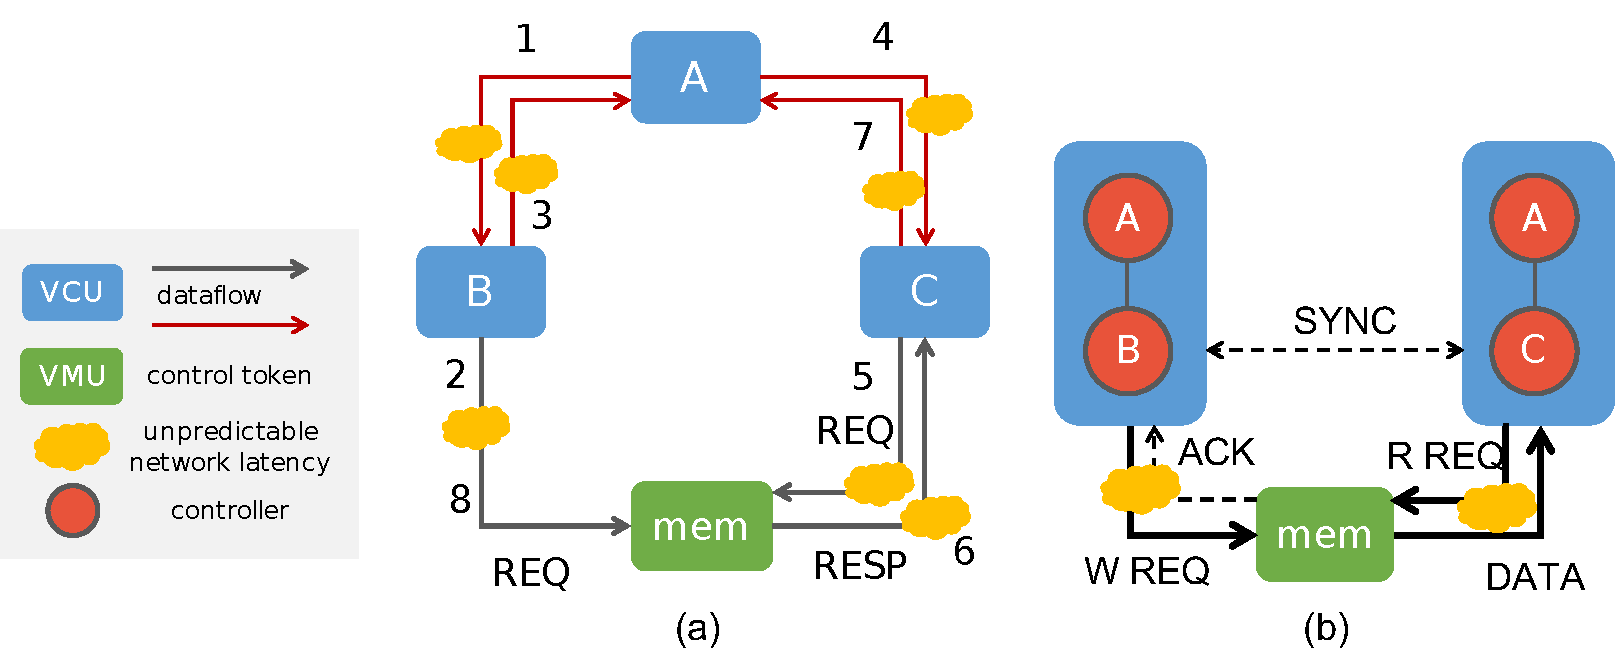
\includegraphics[width=0.8\textwidth]{figs/centralctrl.pdf}
\caption{
  (a) A na\"ive mapping strategy to map the control hierarchy onto Plasticine.
  All units are distributed across an on-chip network that can introduce unpredictable latency.
  The number on the edges indicate the order of event.
  Here we show a scenario where read requests from \emph{C} do not observe the write requests from
  \emph{B} that appears earlier in the program order due to network latency between \emph{B} and
  \emph{mem}.
  (b) Distributed controllers in \name. Each innermost controller makes a copy of all enclosing
  controllers. The signals from these controller are used to generate synchronization between
  distributed compute unit. To address the problem in (a), the memory also needs to provide an write
  acknowledgment per write request for synchronization.
}
\label{fig:centralctrl}
\end{figure*}

To achieve the same execution schedule on Plasticine in a na\"ive approach, 
we can map each controller in the hierarchy into a PU
, sending control signals to schedule the next level 
controllers distributed in other PUs, as shown in \Cref{fig:centralctrl} (a).
This strategy suffers from the expensive network round-trip delays between the parent and child controllers.
To be scalable at a high clock frequency, Plasticine networks are pipelined at each switch,
introducing multiple cycles of network delay across PUs on the control path.
Therefore, the multi-cycle handshaking signal between the parent and the child can introduce significant pipeline bubbles
that undermines performance.
Additionally, this scheme creates a communication hotspot around the parent controller \emph{A} as
loop \emph{A} gets unrolled, which is devastating for a coarse-grained reconfigurable architecture
like Plasticine that has much less routing resource than a FPGA.
Furthermore, synchronizing the compute only is insufficient to ensure memory effects are observed by
the remotely distributed accessors, as shown in \Cref{fig:centralctrl} (a).

To address this challenge, we want to eliminate any of the centralized schedulers for the outer
controllers.
At high-level, \name achieves this by performing loop division for each outer controller, such that
all innermost controllers are perfectly nested, as shown in \Cref{fig:centralctrl} (b).
\name then allocates synchronization tokens across distributed innermost controllers.
All innermost controllers have their own copies of the outer controllers, which are used
to control when to send and consume the control tokens.
These control token ensures the execution order of the inner controllers is the same as if they are
scheduled by a centralized outer controller. Instead of synchronizing all inner controllers under an
outer controllers, \name only synchronizes the ones accessing the same memory, such as \emph{B} and
\emph{C} in \Cref{fig:spatialegpar}. This limits the synchronization among a small set of distributed nodes, 
making our design much more scalable.

The second challenge in this mapping process is that controllers in the spatial hierarchy
can consume arbitrary amount of compute and memory resources, exceeding the capacity of individual
PUs. For instance, a user might write a memory multiple times throughput the program with writers 
mapped to different PUs. The physical scratchpad, however, only has a single write
port. \name needs to virtualize resources, composing or time sharing them when software usage
exceeding the hardware limit.

\begin{figure*}
\centering
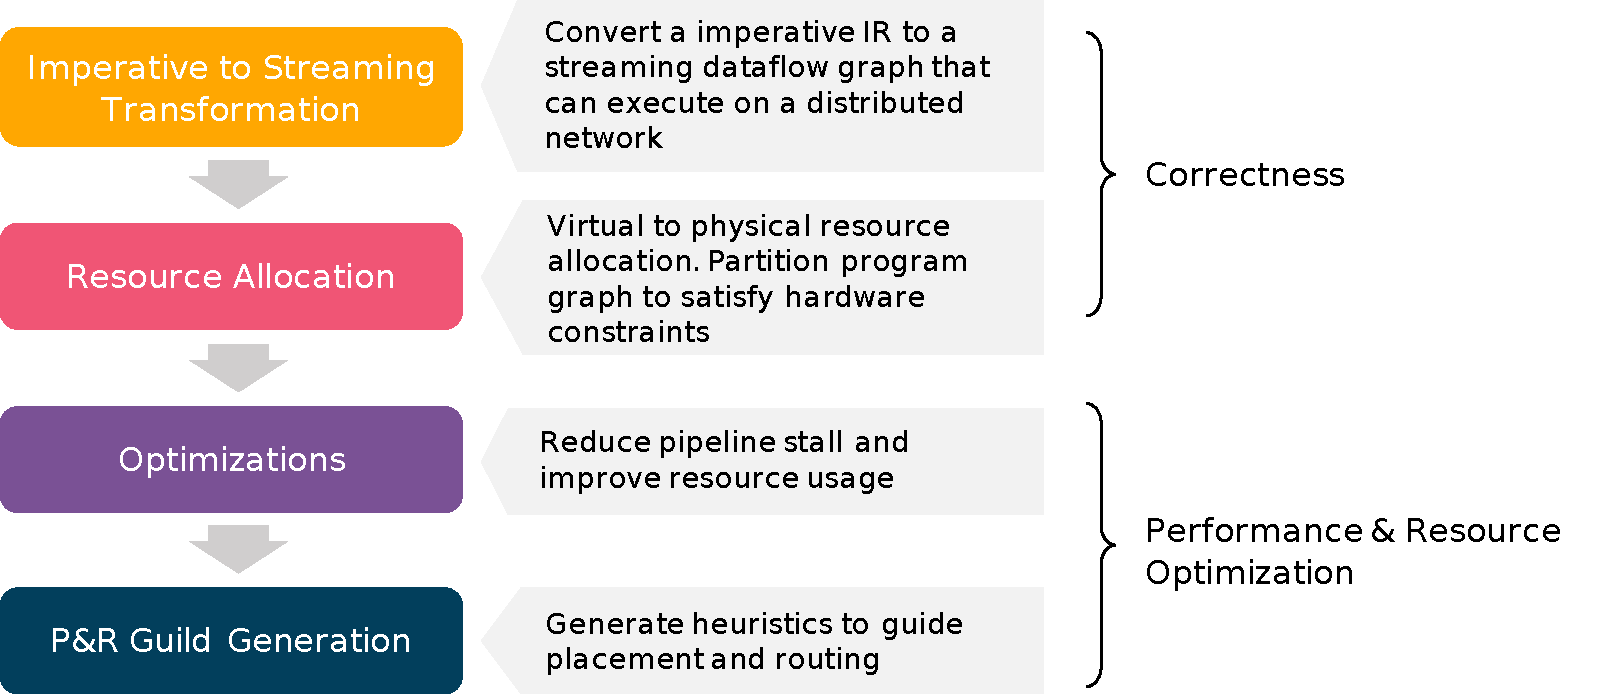
\includegraphics[width=1\textwidth]{figs/sarastack.pdf}
\caption[\name Compiler Flow]{\name Compiler Flow}
\label{fig:flow}
\end{figure*}
 
In the following sections, we describe a systematic approach to compile applications described in an
imperative front-end language to a purely declarative and distributed dataflow graph that can
run on Plasticine. \Cref{fig:flow} shows \name's compilation flow.

\Cref{sec:control} expands on the \term{imperative to streaming transformation} that
addresses the first challenge.
\name allocates distributed on-chip resources to execute the program in spatially parallelized and
pipelined fashion with approperate synchronizations.
A virtual unit (VU) is our intermediate representation that captures computations 
%that will be
%mapped onto 
within the boundary of
a physical unit (PU), such as a PCU and PMU.
Each VU can contain multiple contexts, if their aggregated resources usage can fit in a PU.
The hardware can limit the maximum number of contexts a PU can support and has resources that cannot be split across contexts.
Most importantly, \name needs to ensure messages across VUs, which are mapped across the global network, must tolerate an arbitrary amount of network latencies; messages within a single VU across contexts takes only a single cycle.
The transformation phase generates a virtual unit dataflow graph (VUDFG) with appropriate
synchronizations, such that a streaming pipelined execution over distributed on-chip resources produces the same result as a
parallelized program executed in time.
At the end of the allocation phase, a virtual unit can consume as much resources as the program
requires. 

\name further virtualizes resource allocation and hides the underlying resource constrains on
this hierarchical architecture from the programmers.
\Cref{sec:resalloc} dives into the \term{resource allocation} phase, where \name assign each VU to a
PU that processes the required resources. If no PU can execute a VU, \name partitions the
VU into multiple VUs to eliminate constraint violations. If there is insufficient PU or the VU cannot be partitioned, the mapping process fails with appropriate hints to the programmer for the
limiting resources.

Throughout the first two phases, \name introduces various \term{optimizations} that either reduce the
resource cost of the VUDFG, or alleviates potential performance bottleneck in the streaming
pipeline.
After all VU fits in at least one type of PU, \name performs a global optimization that merges small VUs into a larger VU to reduce resource fragmentations.
\Cref{sec:opt} enumerates the optimizations \name perform.

The output of the resource allocation phase is a VUDFG with a tagged PU type for each VU.
It is up to the
\term{placement and routing (PaR)} phase to determine where the VU will be finally placed.
Right before PaR, \name performs static analysis on the traffic pattern and generate heuristic guild
for the placer to reduce routing congestion.
\Cref{sec:par} details the PaR algorithm and heuristic-guild generated by \name.


\section{Distributed Control Flow}
\label{sec:control}

The input to \name is the backend of the Spatial IR, which is an control hierarchy after loop
unrolling.
The controller at each level of the hierarchy corresponds to a control primitive, such as a loop, or
a branch statement. A basic block is attached to each \emph{inner most} controller including instructions
and memory accesses to user declared data-structures.
\Cref{fig:spatialir} shows an example of a program and a schematic Spatial output IR.

\begin{figure*}
\centering
\begin{subfigure}[b]{0.4\textwidth}
\inputminted{python}{code/spatialeg.py}
\caption{Pseudo Spatial Example}
\end{subfigure}
\hfill
\begin{subfigure}[b]{0.58\textwidth}
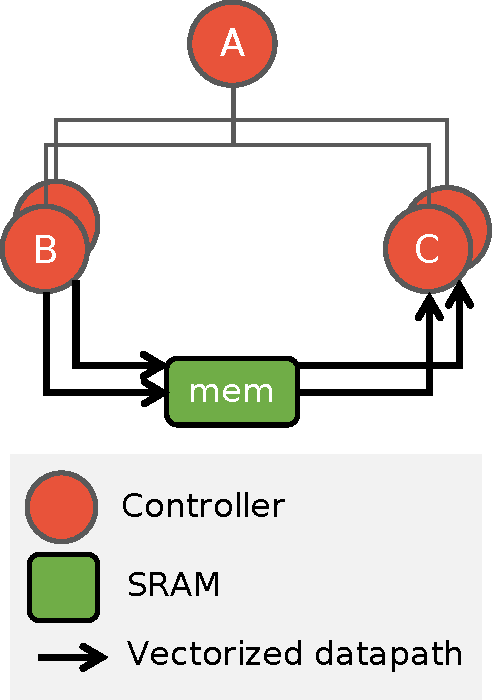
\includegraphics[width=1\textwidth]{figs/spatialir.pdf}
%\missingfigure[figwidth=1\textwidth]{Spatial IR}
\caption{Schematic Spatial IR}
\label{fig:spatialir}
\end{subfigure}
\caption[Spatial Example]{Pseudo example of \name's front-end language}
\end{figure*}

\begin{figure*}
\centering
%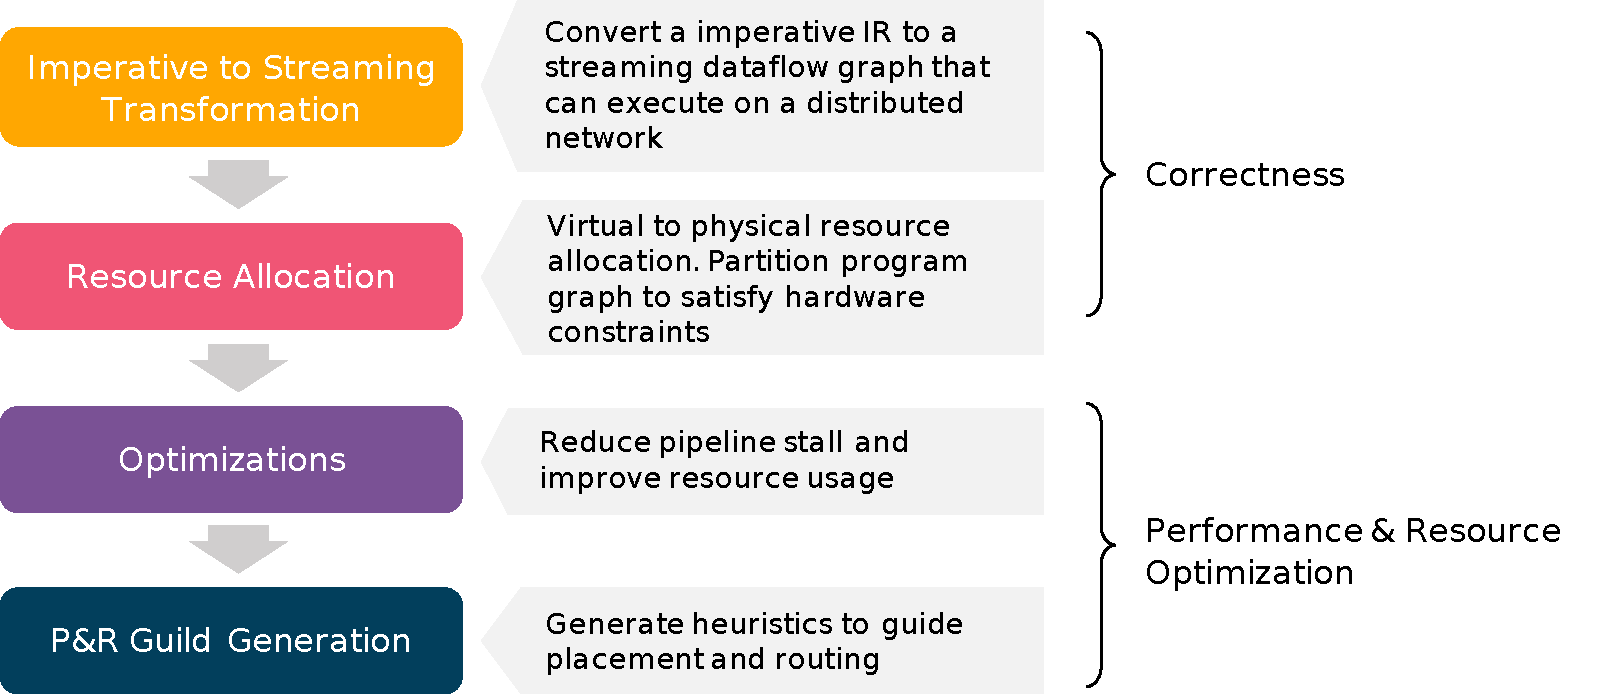
\includegraphics[width=1\textwidth]{figs/sarastack.pdf}
\missingfigure[figwidth=1\textwidth]{Controller duplication}
\caption[Context allocation]{Context allocation}
\label{fig:contextalloc}
\end{figure*}

%\begin{figure*}
%\centering
%\caption[Spatial IR]{Spatial IR}
%\label{fig:spatialir}
%\end{figure*}

As a start, \name allocates one virtual memory to hold each on-chip data structure, and 
one context to execute each basic block within the inner most controllers. 
A basic block maps naturally to a context, as instructions within a basic block are control-free. 
Next, \name makes a copy of all controllers enclosing the basic block in the corresponding context, as
shown in \Cref{fig:contextalloc};
these controllers are later converted to counters and control configurations supported by the
hardware. 
With these controllers, contexts can repeat execution for expected number iterations. However,
data-structures written and read by different contexts are accessed in random order.
The insight is that \emph{as long as all contexts accessing a shared memory with expected program order,
the final result is identical to a sequentially executed program}.
Unlike traditional out-of-order execution, where hardware and compiler look for independent instructions to
execute concurrently, \name starts with all basic blocks executing in concurrent contexts.
\name then introduces synchronizations to maintain consistent access order as expected by the 
program \emph{only} among contexts accessing a shared memory. 
This way, \name introduces minimum p2p synchronizations among small groups of contexts; contexts
accessing different memories are naturally parallelized without impacting the final output.
\todo{walk through an example here}.

To order the execution order or two contexts, \name allocates a single-bit \term{control token} as 
an access grant to the shared memory and passes it between contexts. 
This control token is no different from a regular data-dependency.
By controlling {\em where}, {\em how}, and {\em when} to pass the token, \name 
is able to maintain a consistent update ordering between the pipelined and parallelized actors that access the shared memory.

%In a na\"ive approach, we can map each controller in the hierarchy into a VB (\Cref{fig:centralctrl}).
%This strategy suffers from expensive network round-trip delays between the parent and child controllers.
%If the parent controller is an unrolled loop, the parent needs to synchronize with all child controllers, which creates an undesired communication hot spot.
%\Cref{fig:centralctrl}(a) shows an example where synchronization {\em just} between parent and child controllers can produce an incorrect result due to unpredictable network latency.

%The alternative approach explores a different way to execute the expected control schedule correctly. 
%The minimum required synchronization to produce the correct result is to ensure that the computations access the intermediate results in a consistent matter as if the control schedule is strictly enforced. 
%This can be achieved via p2p synchronizations \emph{only} between computations that access a particular shared memory.
%The execution order of computations that access different memories does not need to be enforced, as they do not impact the program outcome.
%Therefore, as long as the compututation is executed with the expected number of iterations and the memories are updated consistently, there is no need for any extra synchronization.
%Next, we walk through how \name{} achieves this in more concrete detail.


\subsection{Synchronization} 
\label{sec:sync}
We refer to an access to the memory in the input graph as a \emph{declared access}, as supposed to accesses executed at runtime.
For example, multiple accesses across loop iterations are counted as a single declared access.

\paragraph{Where.}
\name only allocate resource to synchronize actors if their declared accesses can potentially interfere.
Whether two declared accesses interfere depends on the type of accesses, the type of the memory, and location of the accesses in the control hierarchy.
For every declared access, \name{} checks other accesses of the same memory appeared earlier in the program order for a possible forward dependency, and later in the program order for a possible loop-carried dependency (LCD). 
Two declared accesses A and B have no dependency if their least-common ancestor (LCA) controller executes only one of the children at anytime (from a branch), or all children in parallel (from an unrolled loop).
The LCD exists between B to A, if B occurs later in the program order, and A and B are surrounded by a loop.
To detect LCD, \name checks if a loop exists among two accesses' LCA controller and LCA's ancestor controllers.
For a dual-ported SRAM, all other accesses need to be synchronized to: share address ports for read-after-read (RAR) and write-after-write (WAW); 
enforce true data-dependency for read-after-write (RAW); and
prevent the overriding of read data for write-after-read (WAR).
\gist{If the memory is multi-buffered (by the user or high-level compiler), we do not need to synchronize for WAR~\cite{dhdl} (the writer writes to a different buffer than the reader does). }
The DRAM interface permits concurrent read streams and, hence, RAR does not need to be synchronized.

\begin{figure*}
\centering
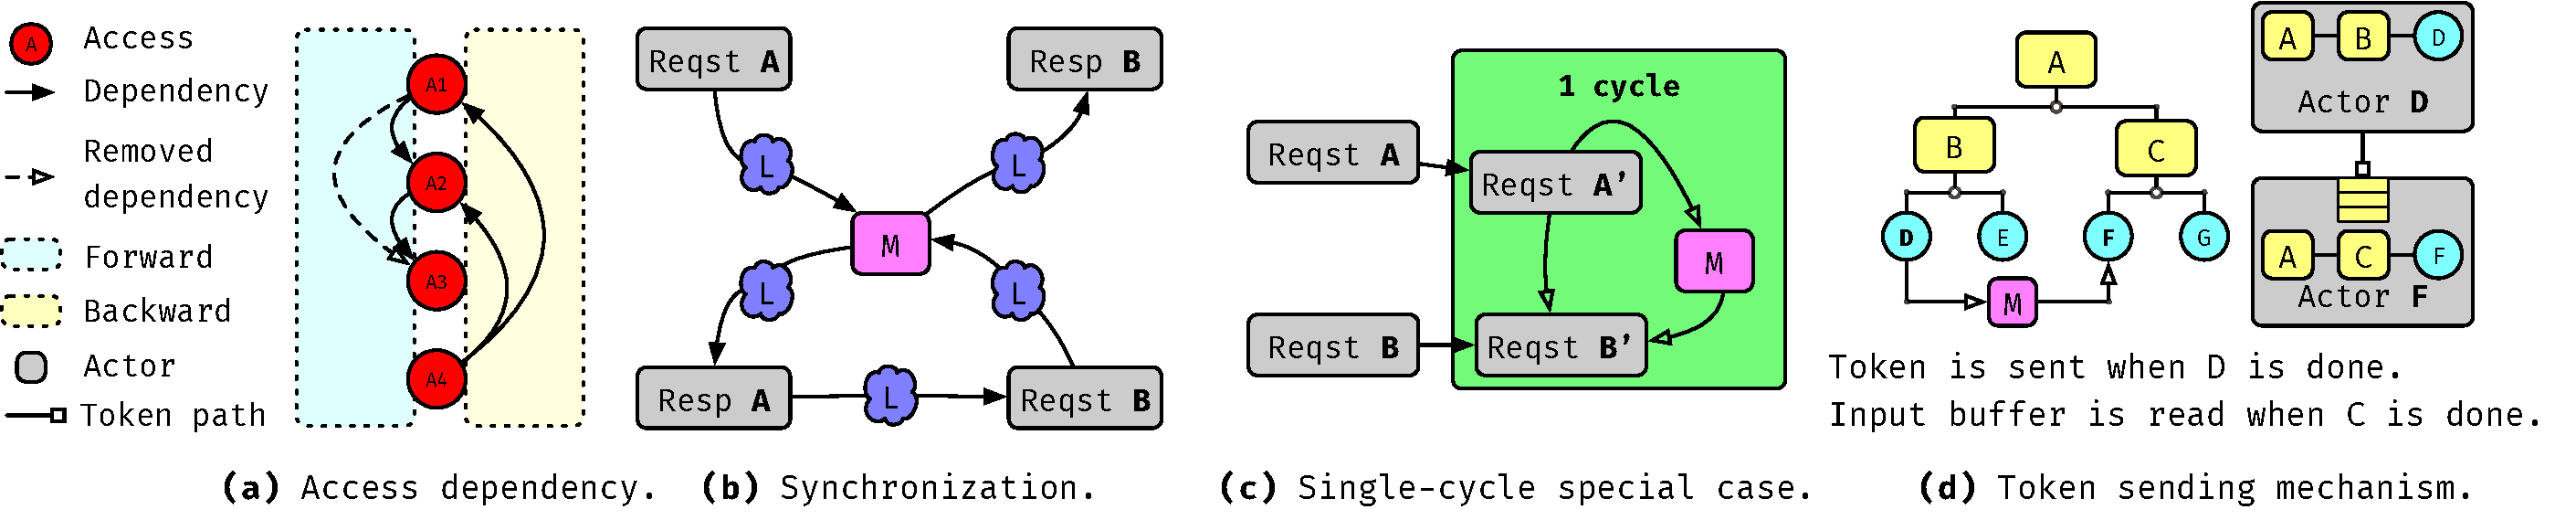
\includegraphics[width=1.0\textwidth]{figs/synch_mech.pdf}
\caption{
    (a) Access dependency graph.
    (b) Synchronization of two accesses on the same memory.
    (c) Single-cycle special case.
    (d) Actors uses local states of controller hierarchy to determine when to send a token.
}\label{fig:depgraph}\label{fig:token}\label{fig:tokentrick}\label{fig:tokenwhen}
\end{figure*}
%\ms{repeated caption, rather give a single caption.}

\paragraph{How.} For each intermediate memory, \name{} builds a dependency graph for all its declared accesses (\Cref{fig:depgraph}(a)).
Enforcing all dependencies in this graph may not be necessary as dependencies between $A_1$ and $A_2$, and $A_2$ and $A_3$ already capture the dependency between $A_1$ and $A_3$.
Therefore, \name{} performs a transitive reduction (TR) on the graph to keep the minimum number of dependency edges that preserve the same ordering \cite{tr}.
Since TR on a cyclic graph is NP-hard, we perform TRs on the forward and backward LCD graphs, separately.
Notice, dependencies between accesses touching different buffers of a multi-buffered memory is less rigid than accesses touching the same buffer.
Therefore, we can only remove an edge if all dependencies on the equivalent path have a stronger or equivalent dependency strength than the strength of the removed edge.

To eliminate the round-trip overhead between the memory and the computation, 
\name{} duplicates the local states and expressions required to generate the requests in a separate actor as the one that handles the responses.
For write accesses, the memory provides an acknowledgment for each request received, used by \name for synchronization.
The request actor generates requests asynchronously as soon as its data-dependencies are cleared, pushing all requests to memory until back-pressured.
To order a declared access A before a declared access B
\name creates a dummy dependency between the actor that accumulates the response of access A ($resp_A$) and the actor that generates requests for access B ($reqst_B$) (\Cref{fig:token}(b)).
To enforce LCD from access B to access A, \name introduces a token from $resp_B$ to $reqst_A$, and initializes the token buffer (input buffer receiving the token) with one element to enable the execution of the first iteration.
If the LCD is on a multi-buffered memory, the LCD token is initialized with the buffer depth number of elements to enable A for multiple iterations before blocked by access B.

These are general schemes we use on any types of memory (including DRAM and on-chip memories) with unpredictable access latency.

\subparagraph{Special Case: Single-Cycle Access}
For a memory with guaranteed {\em single-cycle} access latency, such as registers and statically banked SRAMs that are guaranteed conflict-free, we can simplify the necessary synchronization (\Cref{fig:tokentrick}(c)).
Instead of synchronizing between $resp_A$ and $reqst_B$, we allocate two stateless actors $reqst_A'$ and $reqst_B'$ within {\emph the same} VB as the accessed memory that forwards requests from $reqst_A$ and $reqst_B$, respectively.
Next, we forward the token going from $reqst_A$ to $reqst_B$ to go through $reqst_A'$ to $reqst_B'$ instead, and configure the token buffer in $reqst_B'$ with the depth of one for serialized schedule and depth of M for multi-buffered schedule. 
We no longer need to insert the LCD token, as the stiff back pressure from the token buffer in $reqst_B'$ will enforce the expected behavior.
This optimization only works if the sender and receiver of the token buffer are physically in a single VB where the memory is located.
In this way, when $reqst_B'$ observes $reqst_A'$s token, $reqst_B'$ is guaranteed to observe the memory update from $reqst_A'$ because the memory also has single-cycle access latency.

\subparagraph{Memory Localization}
We perform another specialization on non-indexable memories (registers or FIFOs), whose all accesses have no explicit read enables.
Instead of treating them as shared memories, \name{} duplicates and maps them to local input buffers in all receivers, no longer requiring tokens.
The sender actor pushes to the network when the token is supposed to be sent, and the receiver dequeues one element from the input buffer when the token is supposed to be consumed.
This dramatically reduces the synchronization complexity of non-indexable memory in the common case.

\paragraph{When.}
\name{} configures the actors to generate the token using their local states at runtime.
For FIFOs, the token is generated and consumed every cycle when the producer and receiver actors are active.
For register, SRAM, and DRAM the program order expects that the producer and consumer writes and inspects the memory once per iteration of their LCA controller, respectively.
Since the producer and receiver both have their outer controllers duplicated in their local state, they have independent views for one iteration of the LCA controller, which is when the controller in their ancestors (that is the immediate child of the LCA controller) is completed (\Cref{fig:tokenwhen}(d)).
The {\em done} signals of these controllers are used to produce and consume the token in actors, independently.

\subsection{Data-Dependent Control Flow}
Using the synchronization discussed in \Cref{sec:sync}, we can support control constructs that typically are not supported on most RDAs, such as branch and a while convergence loop.
The controllers in the input graph can also have data dependencies, such as loop ranges. 
The dynamic-loop ranges are handled as data dependencies to actors with \emph{memory localization} described in \Cref{sec:sync}.
The branch condition is also treated as a data-dependent enable signal of controllers under branch clauses.
If the controller is disabled, it is considered {\em done} immediately.
Output tokens depending on the {\em done} signal will be immediately sent out.
For a memory written inside a branch statement and read outside the branch (with a branch miss), the writer actor immediately sends out the token to the receiver
as soon as the branch condition is resolved. 
With a branch hit, the controller waits until its inner controller completes before raising the {\em done} signal.
%This way, the 
A similar scheme is used to implement the while loop, where the while condition is a data-dependency of stop signal of controller X. 
The producer of the while condition also consumes its own output as an LCD. 
The condition is then broadcast to all other actors under the same while loop. 
The {\em done} signal of the while loop is raised when the condition's data-dependency evaluates to true.
At this point, actors accessing memory within the while loop will send the token to access actors outside of the while loop, and enable them to access the intermediate memory.

After all actors and shared resources are allocated and synchronized, we simply put each actor and shared resource into their own VBs.
The actors with single-cycle special case (\Cref{sec:sync}) must be put in the same VB as the shared memory.


\section{Resource Allocation} \label{sec:resalloc}

The output of the imperative to dataflow transformation discussed in \Cref{sec:control} is a VUDFG that 
can execute on a Plasticine with physical units (PUs) that have infinite resources.
The \emph{Resource Allocation} phase enforces and addresses constraint violations given 
the specification of the Plasticine units. 
At the end of this phase, \name assigns each VU in the VUDFG graph to a PU type with required
resources; the placer then takes the type assignments and determines the final placement.

Accelerators often have heterogeneity in compute resources to improve efficiency for common
special operations.
In Plasticine, PMUs and AGs have specialized compute pipelines for address calculation that are 
less capable than the compute pipeline in PCUs.
However, heterogeneity tends to reduce average utilization because different applications, and even the same application with different data sizes, can vary highly in the desired ratio among different
resource~\cite{tz_rnn}.
A compute-bound application, for example, can heavily underutilize the AGs and PMUs.
To address this problem, \name models the virtual to physical assignment as a constraint satisfaction problem; 
each VU consumes a set of resources and can only be assigned to a PU if the PU processes the required resources. 
%Instead of using heuristics to assign certain a type of VU to a type of PU, we
\Cref{tab:resource} shows the types of resources \name models in Plasticine's heterogeneous units.
For example, special connection to off-chip memory interface is
also treated as a type of resource in the AG, which forces virtual contexts accessing DRAM to map to AGs. 
On the other side, regular contexts with non-vectorized fixed-point operations can also be mapped to
spare AGs, which improves utilization.
\begin{table*}
  \centering
\begin{tabular}{lccccc}
  \toprule
  Feature & PCU & PMU & AG & Host Unit & Aggregation Function\\ \midrule
  Vector lane width & 16 & 16 & 1 & 1 & \multirow{2}{*}{MAX}\\
  \# pipeline register (PR) & 8 & 8 & 4 & 0 & \\ \hline
  \# stages & 6 & 10 & 5 & 0 & \multirow{6}{*}{SUM}\\
  Scratchpad banks & 0 & 16 & 0 & 0 &  \\
  Scratchpad capacity & 0 & 256kB & 0 & 0 & \\
  MergeBuffer & 1 & 0 & 0 & 0 & \\
  Splitter & 1 & 0 & 0 & 0 & \\
  Scanner & 1 & 0 & 0 & 0 & \\ \hline
  Operation types & fix $\cup$ float & fix & fix & $\varnothing$ & $\cup$ \\ \hline
  Reduction tree & \cmark & \xmark & \xmark & \xmark & \multirow{3}{*}{OR}\\
  Access to DRAM Interface & \xmark & \xmark & \cmark & \xmark & \\
  Access to Host IO & \xmark & \xmark & \xmark & \cmark & \\ \hline
  \# Vector Input & 6 & 6 & 4 & 0 & \multirow{6}{*}{G}\\
  \# Scalar Inputs & 6 & 6 & 4 & 16 & \\
  \# Control Inputs & 16 & 16 & 4 & 16& \\
  \# Vector Outputs & 6 & 6 & 4 & 0 & \\
  \# Scalar Outputs & 6 & 6 & 4 & 16 & \\
  \# Control Outputs & 8 & 8 & 2 & 16 & \\
 \bottomrule
\end{tabular}
\caption[Resources specification of heterogeneous units and aggregation function]{
  A list of resources \name models in four types of configurable units in Plasticine. The host unit
  models the host registers I/Os.
  MergeBuffer, Splitter, and Scanner are new hardware units introduced in \cite{gorgon} and recent work
  to support database and sparsity in Plasticine.
  The aggregation function indicates how to compute the aggregated resource cost when two contexts are merged
  into a single virtual unit (VU). G indicates the aggreated value is the output of a graph traversal of the
  merged graph. How to count \# I/O is discussed later in \Cref{sec:compsplit}.
  While the aggreation function of \#PR of two merged contexts is MAX, the \#PR of a
  context is the maximum number of live variables of its dataflow graph, which is also an output of
  a topological traversal.
  This table reflects a different Plasticine configuration as the original Plasticine in \cite{plasticine}.
}
\label{tab:resource}
\end{table*}

\begin{algorithm}
  \Fn(\tcc*[h]{Allocation Algorithm}){alloc(V, P, pruners)}{
    \KwData{V: a set of VUs from the VUDFG}
    \KwData{P: a set of all PUs on the hardware}
    \KwData{pruners: a list of constraint pruners to check
    and fixes constraint violations}
    \tcc{Initialize a complete bipartite graph}
    G = \KwNew BipartiteGraph()\;
    G[V] = P\;
    \tcc{Constraint resolution}
    prune(G, pruners)\;
    \tcc{Global merging}
    merge(G)\;
    \tcc{Heuristic check on whether assigning all VUs in V is feasible}
    check(G)\;
    \tcc{Virtual to physical assignment}
    backtracking\_assign(G)\;
  }
  \vspace{0.5cm}
  \Fn(\tcc*[h]{A recursive pruning function}){prune(G, pruners)}{
    \KwData{G: bipartite graph between VUs and PUs}
    \KwData{pruners: a list of constraint pruners to check
    and fixes constraint violations}
    \KwResult{The function update G by removing VU-PU edges that violates constraints guarded by
    pruners. The function may fail and raise an exception.}
    \tcc{All PUs on the hardware}
    P = G.values()\;
    \For{pruner \KwTo pruners}{
      \For{v \KwTo G.keys()}{
        \For{p \KwTo G[v]} {
          \If{pruner.cost(v) > pruner.cost(p)} {
            G[v] -= p\;
          }
        }
        \If{G[v].empty()} {
          \tcc{Partition VU v based on resource constraints registered in pruner. 
          Not all resources can be partitioned and this step may fail.
          If succeeded, the function returns a new set of VUs.}
          V' = pruner.partition(v)\;
          G' = \KwNew BipartiteGraph()\;
          G'[V'] = P\;
          prune(G',pruners)\;
          G -= v\;
          G[V'] = G'[V']\;
        }
      }
    }
  }
  \caption{Resource allocation. The bipartite graph \texttt{G} contains a bi-directional many-to-many
  map. \texttt{G[key]} returns the set of values connecting to the key (dom(key)), and \texttt{G[value]}
  returns the set of keys connecting to the value.
  \texttt{G[key] = value} connects an edge between key and value.
  \texttt{G[KeySet] = ValueSet} creates all-to-all connection between \texttt{KeySet} and
  \texttt{ValueSet}.}
  \label{algo:resalloc}
\end{algorithm}

\begin{algorithm}
  \Fn(\tcc*[h]{Assignment feasibility check}){check(G)}{
    \KwData{G: bipartite graph}
    \KwResult{Whether it is possible to assign all VUs in V with a different PU in P}
    \tcc{For every value set in \texttt{G}}
    \For{V \KwTo G.values().toSet()} {
      K = $\varnothing$\;
      \For{v \KwTo V} {
        \For{k \KwTo G[v]} {
          \If{G[k] $\subset$ V} {
            K += k\;
          }
        }
      }
      \If{|K| > |V|} {
        \KwRet{failure()}\;
      }
    }
    \KwRet{success()}\;
  }
  \caption{Heuristic check on whether it is possible to assign all key with an value in a bipartite
  graph. Given there are only a few types of hardware tiles, $G.values().toSet()$ is
  relatively small. This algorithm roughly runs in $O(|G.keys()|\times|G.values()|)$, which is
  still much faster than the backtracking assignment with exponential runtime.}
  \label{algo:check}
\end{algorithm}
 
%% backtracking_assignment(vu, dom)
As shown in \Cref{algo:resalloc}, the \emph{resource allocation} phase contains three steps:
\emph{constraint resolution}, \emph{global merging}, and \emph{virtual to physical assignment}.
\name uses a VU-PU bipartite graph (\emph{G}) to keep track of potential valid assignments between the two.
Initially, \emph{G} is initialized to a complete bipartite graph, i.e., all VUs can be assigned to
all PUs.
We refer to all PUs connected to a VU \emph{v} as the domain of \emph{v} in G, i.e. \emph{dom(v)}.

\paragraph{Constraint Resolution}
A list of constraint pruners, each considering a set of on-chip resources, 
incrementally remove the VU-PU edges that violate the resource constraints.
If a VU \emph{v} has an empty domain after pruning, the pruner attempts to fix the violation by
decomposing the VU into multiple VUs. 
Not all resources are composable, and the partitioning transformation may fail.
If succeeded, the partitioner generates a new set of VUs \emph{V'}. \name starts a new complete bipartite
graph between \emph{V'} and all resources \emph{P}, and recursively prune on \emph{V'}.
If succeeded, the original graph \emph{G} is updated with \emph{V'} and their pruned resources.

\paragraph{Global Merging}
After all VUs have at least one PU in the bipartite graph, \name triggers a global optimization that merges 
small VUs into a larger VU to reduce fragmentation in allocation.
Each type of resource has an aggregation rule to compute how the resource cost changes if two VUs are merged
together, as shown in \Cref{tab:resource}. 
Most aggregation rules are simple, such as addition, logical or, max, or union.
The in- and out-degree costs are tricker and will be detailed in \Cref{sec:compsplit}.

\paragraph{Virtual to Physical Assignment}
Next, \name performs a quick heuristic check on the bipartite graph to see if there exists a
possible assignment for all VUs with sufficient PUs (\Cref{algo:check}), and provide feedback on the limiting resources, otherwise.
Finally, \name assigns each VU to a PU type with a backtracking search on the pruned bipartite
graph.

This approach can be easily extended to handle new heterogeneous tiles in the architecture by registering
the tile with existing or new types of resources with aggregation and partitioning rules.
The rest of this section goes over two types of partitioning transformations--compute
partitioning in \Cref{sec:compsplit} and memory partitioning in \Cref{sec:memsplit}.
%We have another partitioner encoding valid rule to decompose a BlackBox IP block available on the RDA.

\subsection{Compute Partitioning} 
\label{sec:compsplit}

The {\em compute-partitioning} phase addresses VUs using more compute resources than any PU can provide. 
If a VU contains multiple contexts, \name{} first moves the contexts into separate VUs.
If a single context exceeds the resource limit, \name breaks down the dataflow graph in the context into multiple contexts and puts them in separate VUs.
During partitioning, \name maps each subgraph of the large dataflow graph into a new context, mirrors the control states of the original context, and streams live variables in between.
We can formulate the problem of how to partition in the dataflow graph as an optimization problem, shown in
\Cref{tab:partprob}.
The partitioner ``fixes'' the VU \emph{v} based on a single PU specification, albeit there are many potential PUs 
the decomposed VU can be mapped to.
Currently, we use a heuristic to select a PU type from \emph{dom(v)} right before the compute pruning 
as a guiding constraint for partitioning.

\begin{table*}
  \centering
\begin{tabular}{lp{12cm}}
  \toprule
  \textbf{Problem} & Partition the dataflow graph into subgraphs such that all subgraphs satisfy the constraints of a
  hardware unit. \\[0.9cm]
  \textbf{Objective }& Minimize the number of partitions and connectivity across partitions. \\[0.5cm]
  \textbf{Constraints} & 
  \begin{minipage}{12cm}
  \begin{outline}
  \0 Each partition must not exceeds the limit on the number of \vspace{-0.2cm}
    \1 live in/out variables (I/O ports) \vspace{-0.2cm}
    \1 operations (pipeline stages), \vspace{-0.2cm}
    \1 and live variables across operations (pipeline registers), etc.\vspace{-0.2cm}
  \0 No \emph{new} cycles can form across partitions other than the cycles in the original
  dataflow graph.
  \end{outline}
  \end{minipage}
  \\
 \bottomrule
\end{tabular}
\caption[Formulation of the compute partitioning problem]{
Formulation of the compute partitioning problem
}
\label{tab:partprob}
\end{table*}

Because the global network is specialized to handle efficient broadcasts, 
the in/out-degree of a partition counts the number of unique live-in/out variables, as supposed to
the number of edges across partitions.
In addition, the partitioned subgraphs cannot form {\em new} cycles; contexts waits for all
input dependencies and therefore cycles across contexts cause deadlock. 
Nonetheless, the original graph might contain cycles representing loop-carried dependencies, such as
accumulation. For these cycles, \name initializes the back edge of the cycle with dummy data to
enable execution.
\Cref{fig:parteg} shows examples of valid and invalid partitioning solutions.
\Cref{fig:partcycleeg} shows another partitioning example of a dataflow graph with cycles.

\begin{figure}
  \centering
  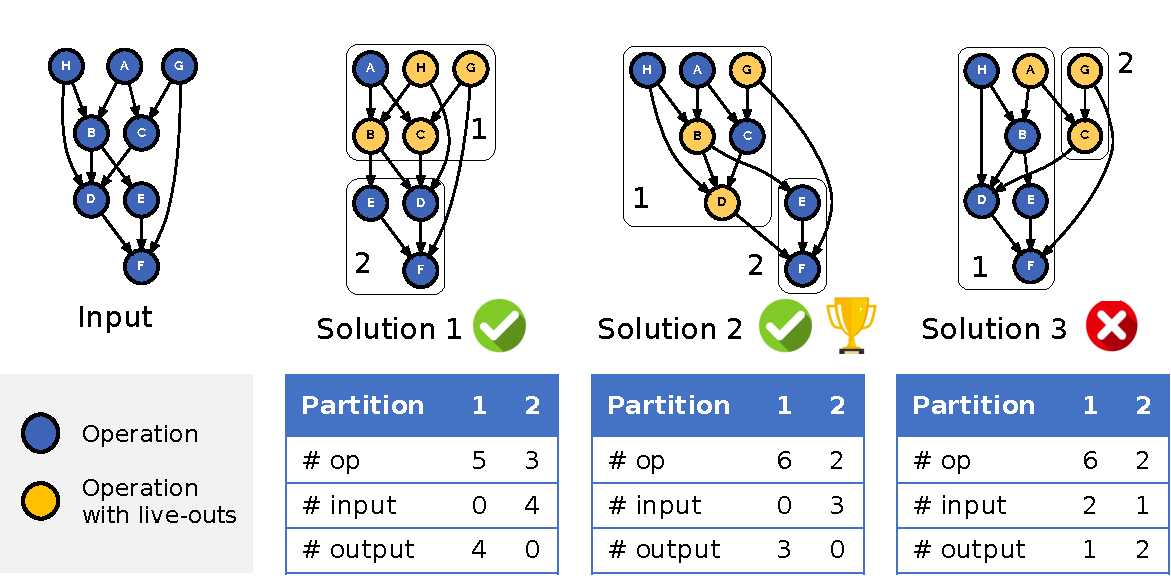
\includegraphics[width=1\columnwidth]{figs/parteg.pdf}
  \caption[Compute partitioning examples]{
    Compute partitioning examples. Solution 1 and 2 are both valid. Solution 2 is
    better because it has less number of broadcast edges across partitions (3 as supposed to 4 in Solution 1). 
    Solution 3 is an illegal partitioning due to the cycle between partition 1 and 2.
  }
  \label{fig:parteg}

  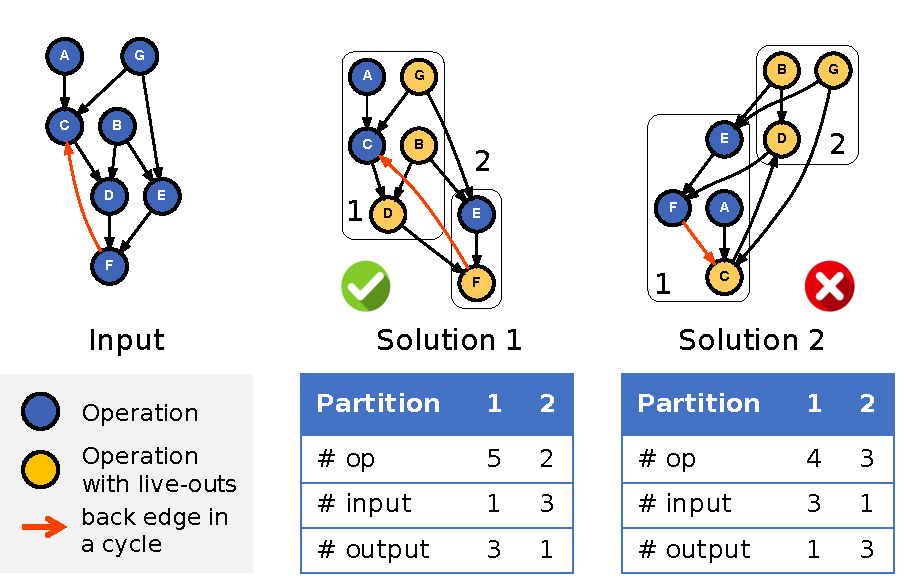
\includegraphics[width=0.8\columnwidth]{figs/partcycleeg.pdf}
  \caption[Compute partitioning examples with cycle]{
    Compute partitioning examples with cycle in the dataflow graph.
    Solution 1 is valid because there is no 
    cycle between partitions after removing the back edge in
    the original graph.
    Solution 2 is invalid because there is still cycle between partition 1 and 2 after
    removing the back edge.
  }
  \label{fig:partcycleeg}
\end{figure}

\paragraph{Community Detection}
The formulation of compute partitioning is similar to the community detection
problem\cite{community} that has a similar objective. 
The major difference is that the latter often takes the number of output partitions as an
input to the algorithm, whereas our problem partitions until all subgraphs satisfy all constraints.
Moreover, community detection algorithms do not enforce the cycle constraints. 
Finally, the edge connectivity in community detection counts the number of edges across partitions, 
as supposed to broadcast edges as in our problem.

\paragraph{Retiming}
Imbalanced data paths across partitions can cause pipeline stalls at runtime if the long-live path is not
sufficiently buffered.
To ensure full-throughput pipelining, \name needs to insert retiming buffers along the imbalanced data path across
partitions.
Retiming introduces new VUs in addition to the partitioned VUs, which attributes to the cost in
\Cref{tab:partprob}'s objective.

In the following sections, we present two algorithms to resolve the problem described in
\Cref{tab:partprob}:
a fast traversal-based algorithm providing a decent solution, and a slow convex
optimization-based algorithm providing an optimal solution.

\subsubsection{Traversal-based Solution}
To address the cycle constraint, the traversal-based algorithm performs a topological sort of the dataflow graph.
The topological sort ignores the back edges of the cycles during traversal. 
Starting from one end of the sorted list, the algorithm iteratively adds nodes into a partition
until it fits no more nodes. The algorithm then repeats the process with a new partition.
This approach guarantees that no cycle is introduced with $O(V+E)$ complexity, 
where $V$ and $E$ are the numbers of vertices and edges in the dataflow graph.

The partitioning result is a function of the traversal order.
We experienced with depth-first search (DFS) and breadth-first search (BFS) with forward and
backward dataflow traversal orders.
For DFS, we re-sort the remaining list each time starting with a new partition.

\subsubsection{Solver-based Solution}
The convex optimization solution models the problem as a node-to-partition assignment problem.
\Cref{tab:solver-eqns} gives our formulation and \Cref{tab:solver-variables} explains the notations
used in \Cref{tab:solver-eqns}.

\begin{table*}
  \centering
	\begin{tabular}{c | c | c | c}
		\textbf{Name} & \textbf{Type} & \textbf{Description} & \textbf{Definition / Default}\\\hline
		$\mathcal{N}$ & Constant & Enumeration of nodes to partition, numbered $\{n_i\}_i$ & - \\
		N & Constant, $\nnint$ & Number of operations to partition & $N = |\mathcal{N}|$\\
		P & Constant, $\nnint$ & Number of partitions to consider & $N$, or from heuristic \\
		$\mathcal{E}$ & Constant, $\{n_i \to n_j\}$& Directed edges representing dependence & - \\
		B & Variable, $\{0, 1\}^{N \times P}$ & Boolean Partitioning Matrix& - \\
		%p & Variable, $\nnint^N$ & Vector of mappings from node to assigned partition& $p = B \begin{bmatrix} 0 & 1 & \cdots & P-1\end{bmatrix}^T$\\
		$\projb{\cdot}$ & $\nnint \to \mathbb{B}$ & Function to convert a positive integer into a boolean& Supplemental Materials\\
		$\andf(\cdot, \cdot)$ & $\{0, 1\} \times \{0, 1\} \to \{0, 1\}$ & Boolean and of binary variables & Supplemental Materials \\ 
		$d_p$ & Variable, $\nnint^P$ & Vector of partition delays & - \\
		$d_n$ & Variable, $\nnint^N$ & Vector of node delays & - \\
		$\dest(n)$ & $\mathcal{N} \to \mathcal{P}(\mathcal{N})$& The set of nodes which depend on $n$& $\{n' | n' \in \mathcal{N}\ s.t.\ (n \to n') \in \mathcal{E}\}$\\
		$c_o$ & Constant, $\nnint$ & Maximum output arity of a partition & HW Spec \\
		$c_i$ & Constant, $\nnint$ & Maximum input arity of a partition & HW Spec \\
		$b_d$ & Constant, $\nnint$ & Maximum input buffer depth & HW Spec \\
		$K$ & Constant, $\mathbb{R}_+$ & Very Large Constant, used for constraint activation & $P \times N$ \\
		$\alpha_d$ & Hyperparameter, $\mathbb{R}_+$ & Retime merging probability multiplier& $\frac{1}{\max\{c_o, c_i\}}$ \\
	\end{tabular}
	\caption{Names and definitions used in the solver-based partitioning.}
	\label{tab:solver-variables}
\end{table*}

\begin{table*}
  \centering
  \newcommand\cola{1.6cm}
  \newcommand\colb{3.8cm}
  \newcommand\colc{9cm}
  \newcommand{\gcell}[2]{\Gape[#1cm][0cm]{\makecell[l]{#2}}}
  \begin{tabularx}{\textwidth}{cp{\colb}X}
    \toprule
		\textbf{Type} & \textbf{Description} & \textbf{Expression}\\\midrule
    \multirow{3}{*}{\makecell[l]{Cost\\Function}} & Allocated Partitions & $\Sigma_i \projb{\Sigma_j B_{i, j}}$\\

    & \makecell[l]{Additional Retiming\\Partitions}
    & $\alpha_d \Sigma_{n_i \to n_j \in \mathcal{E}} \projb{\max\{d_n(j) - d_n(i) - b_d, 0\}}$\\[0.3cm]
		\hline

    \multirow{12}{\cola}{\makecell[l]{\\\\Constraint}} & Partition Assignment & $ \forall n_i \in \mathcal{N}:\ \Sigma_j B_{i, j} = 1$\\[0.1cm]

    &\makecell[l]{Dependency\\Constraint} & $\forall n_i \to n_j \in \mathcal{E}:\ d_n(i) + 1[p_i \ne p_j] \le d_n(j)$\\[0.1cm]

    &\makecell[l]{Output Arity\\ Constraint} 
    &\makecell[l]{
      $\forall p \in [0, P):$ \\
      $\Sigma_{n_s \in \mathcal{N}} \andf(B_{s, p}, \projb{\max\{(\Sigma_{n_d \in \dest(n_s)} B_{d, p}) -$ \\
      $K \times B_{s, p}, 0\}}) \le c_o$
    }\\[0.7cm]

    &\makecell[l]{Input Arity Constraint\\ (vectorized)} & $\Sigma_{n_i \in \mathcal{N}} \max\{\projb{\Sigma_{n_j \in \dest(n_i)} B_{j, :}} - B_{i, :}, 0\} \le c_i \times \vec{1}$\\

		&Delay Consistency& 
    \makecell[l]{
    $\forall n_i \in \mathcal{N}:\ d_n(i) \le \min_j (d_p(j) + K - B_{i, j} \times K)$ \\
		$\forall n_i \in \mathcal{N}:\ d_n(i) \ge \max_j (d_p(j) + B_{i, j} \times K - K)$
    }\\[0.5cm]

		&Constant Validity& 
    \makecell[l]{
      $\forall n_i \in \mathcal{N}:\ d_n(i) \le K$\\
		  $\forall i \in [0, P):\ d_p(i) \le K$
    } \\
    \bottomrule
	\end{tabularx}
  \caption{Solver formulation for partitioning*.}
	\label{tab:solver-eqns}
\end{table*}

\begin{table*}
	\begin{tabular}{c | c | c | c}
		\textbf{Name} & \textbf{Type} & \textbf{Description} & \textbf{Definition / Default}\\\hline
		$\mathcal{C}_r$& $[\mathcal{N} \to \mathbb{R}_+,\mathbb{R}_+, [\mathbb{R}_+] \to \mathbb{R}_+]$ & List of per-node values, limits, and reduction& Supplemental Materials\\&& functions for reducible constraints& \\
		F & $\{0, 1\}^{N \times P}$ & Feasibility matrix, whether a partition can support a node& HW Spec \\ 
	\end{tabular}
	\caption{\Cref{tab:solver-variables} extension for solver-based merging, which is a generalization of the partitioning problem.}
	\label{tab:merging-variables}

	\begin{tabular}{c | c | c}
		\textbf{Type} & \textbf{Description} & \textbf{Expression}\\\hline
		Constraint & Feasibility Constraint & $ \forall i, j \in [0, N) \times [0, P):\ B_{i, j} \le F_{i, j}$\\
		& Reducible Constraints & $\forall j \in [0, P).\ \forall (c(\cdot), c_v, r(\cdot)) \in \mathcal{C}:\ r([c(n_i) \times B_{i, j}]_{n_i \in \mathcal{N}}) \le c_v$\\
	\end{tabular}
  \caption{\Cref{tab:solver-eqns} extension for solver-based merging*. The Retiming Partition objective is not used for merging.}
	\label{tab:merge-eqns}
  \scriptsize
  \raggedright
  \vspace{-0.3cm}
  *Expressions are presented using the Disciplined Convex Programming ruleset \cite{DCP, DCP-online}. Explanations for selected expressions can be found in the supplemental material.
\end{table*}



At a high-level, we use a boolean matrix $B$ to keep track of the assignment. 
$B$ has dimension equals to the number of nodes in the dataflow graph by the maximum number of partitions, where$B[i,j]=1$ 
indicates node $i$ is assigned to partition $j$.
In \Cref{tab:solver-eqns}, \emph{partition assignment} restricts each node to have a single partition assignment.
The \emph{input and output arity constraints} show the formulations that limit the number of input
and output for a subgraph.
These are the two most challenging constraints as we need to identify broadcast edges across partitions.
To address the cycle constraint, we introduce a delay vector $d_n$ with a size equivalent to the number of nodes. 
The delay vector encodes a time schedule to execute each node, whose values are selected by the solver.
The \emph{dependency constraint} enforces a node can be scheduled no earlier than its input dependencies and
no later than its output dependents.
Since the operations within a partition have to be triggered atomically, there is another delay
vector $d_p$ for partitions. The \emph{delay consistency} enforces the schedule of a node equals to the
schedule of its assigned partition.
Finally, \emph{constant validity} limits the range of values the delay vectors can be chosen from.
In addition to enforcing the cycle constraint, 
these delay variables are also used to calculate where retiming is required and project the amount of introduced retiming VUs. 
Finally, we use the traversal-based solution to warm start the assignment matrix
$B$ and the delay vectors to reduce the solver runtime.

\subsubsection{Comparison}

\begin{figure*}
\centering
\hfill
\begin{subfigure}[b]{0.35\textwidth}
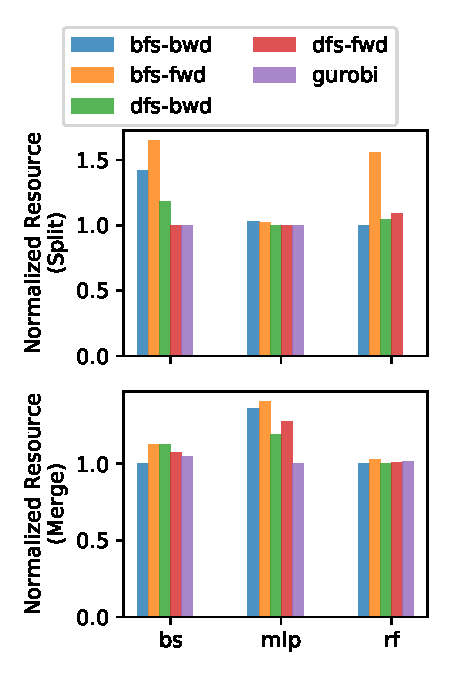
\includegraphics[width=1\textwidth]{figs/algo2.pdf}
\caption{Resource Comparison}
\end{subfigure}
\hfill
\begin{subfigure}[b]{0.64\textwidth}
\centering
\begin{tabular}{lccccc}
  \toprule
  Apps &bfs-bwd & bfs-fwd & dfs-bwd & dfs-fwd & gurobi \\ \midrule 
bs & 3s & 3s & 2s & 2s & 2h4m \\ 
mlp & <1s & <1s & <1s & <1s & 4s \\ 
rf & 1m37s & 1m7s & 29s & 27s & - \\ 

 \bottomrule
\end{tabular}
\caption{
  Compile time for spltting
}
\vspace{0.1cm}
\begin{tabular}{lccccc}
  \toprule
  Apps &bfs-bwd & bfs-fwd & dfs-bwd & dfs-fwd & gurobi \\ \midrule 
bs & 1s & 2s & 5s & 3s & 1m4s \\ 
mlp & 5s & 5s & 6s & 11s & 31m16s \\ 
rf & 11s & 10s & 2m7s & 1m0s & 14h27m \\ 

 \bottomrule
\end{tabular}
\caption{
  Compile time for merging
}
\vspace{0.65cm}
\end{subfigure}
\hfill
\caption[Partitioning and merging algorithm comparisons]{
  Partitioning and merging algorithm comparisons. (a) shows the normalized resource usage between
  different algorithms (the lower the better). (b) and (c) shows the compile time of each algorithm.
  Benchmarks include BlackScholes (bs), multi-layer perceptron (mlp), and random forests (rf).
}
\label{fig:split}
\end{figure*}

\Cref{fig:split} shows the comparison between the traversal-based and the solver-based solutions for both
compute partitioning and global merging.
Global merging is a global optimization merging small VUs into a large VU that can still fit in
a PU. 
The merging algorithm is very similar to the compute partitioning algorithm, where nodes in the
dataflow graph corresponds to the VUs in a VUDFG. 
The traversal and solver-based algorithms for partitioning can be extended to handle the merging
problem.
\Cref{sec:opt} will discuss merging problem in more detail.

We use a commercial solver, Gurobi~\cite{gurobi}, for the solver-based algorithm. 
The evaluation is performed on an Intel Xeon E7-8890 CPU at 2.5GHz with 1TB DDR4 RAM. 
Gurobi is parallelized across ten threads for each application.
To speed up convergence, we configure Gurobi with a 15\% optimality gap, i.e., 
the solver is allowed to early stop after the current solution is less than 15\% worse than the optimum
solution. 
%To speed up convergence, we use a 15\% optimality gap that stops the solver at a reasonable solution.
The solving time increases dramatically as getting close to 100\% optimum.

\Cref{fig:split} (a) shows the normalized resources in the number of VUs after partitioning and merging.
We can see that Gurobi provides almost the best solution for all applications when it can derive
an answer in a reasonable amount of time. The missing solver bar in random forest (\emph{rf}) partitioning
is due to timeout after a few days.
The traversal-based algorithms can sometimes match or even outperform the solver slightly.
However, because the partitioning result is a function of the traversal order, 
each traversal order has adversarial cases, where they can be up to 1.7x worse in resource than the best possible solution.
We found the forward (\emph{fwd}) traversal order schedules nodes as earlier as possible, reducing the number of
external live variables; the backward traversal minimizes the number of internal live variables
across partitions.
The depth-first-search (DFS) traversal order minimizes the number of live variables between partitions, 
albeit producing more imbalanced paths between partitions. 
On the other hand, breath-first-search (BFS) produces more balanced partitioning with more live variables and partitions.

There are two common graph patterns in the applications that require partitioning. 
The first is a dataflow graph from a large basic block, which contains a small set of external
live-in and -out variables and many intermediate temporary variables.
Such graphs typically end up with long-live variables across partitions that require retiming.
%\todo{show example and discuss the other pattern.}
The second is a balanced tree structure as the result of partitioning
a logical memory across PUs discussed later in \Cref{sec:memsplit}.
The first structure favors the DFS traversal order, minimizing the number of partitions. The second
structure favors the BFS traversal order, creating balanced partitions without additional
retiming VUs.

\Cref{fig:split} (b) and (c) shows the compile time for these algorithms. The single-threaded
the traversal-based algorithm runs in minutes, which is significantly faster than the parallelized solver that takes hours to days.
In general, the solver runtime becomes quickly unbounded with a large amount of VUs.
%\todo{show solver time with an increasing number of VBs}.

In summary, the solver solution provides a guaranteed close-to-optimum solution at an expensive
compile time. Nonetheless, the solver-solution treats the retiming and partitioning as a joint optimization,
whereas the traversal-based solution solves these two problems in two separate passes,
generating less optimal solutions.
Moreover, the solver-based solution tends to produce a better result for PUs with a tight I/O
bound (small number of I/Os and large number of stages).
The traversal-based solutions, on the other hand, can produce a decent solution in a short amount of
time.
However, the solution is a function of the traversal order; hence, the quality of the partitioning
is highly sensitive to the graph structures.
In practice, we can combine the two approaches and invoke the expensive solver only when the
traversal-based solution is insufficient. The quality of the traversal-based solution can be easily
estimated with the resource utilization of a partition.

\subsection{Memory Partitioning} \label{sec:memsplit}
The memory pruner addresses virtual on-chip memory exceeding the capacity and bandwidth limit of a
single PMU.
As we parallelize the computation, the on-chip memory must provide higher address bandwidth to sustain the
compute throughput.
On a processor-based architecture, this is often achieved with a separate first-level
cache for each processor core, as shown in \Cref{fig:memmodel} (a).
The cache implements a hardware coherence protocol that synchronizes the different copies of data
behind the scenes,
providing the abstraction of a shared memory.

\begin{figure}
  \begin{subfigure}[b]{0.35\textwidth}
  \centering
  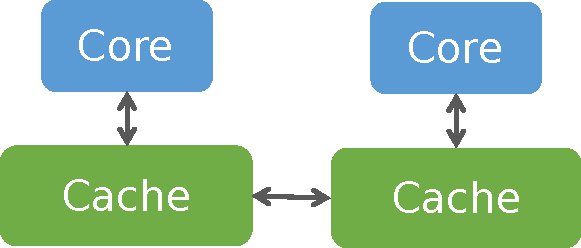
\includegraphics[width=1\columnwidth]{figs/cpumemmodel.pdf}
  \caption{Processor Architecture}
  \end{subfigure}
  \hfill
  \begin{subfigure}[b]{0.45\textwidth}
  \centering
  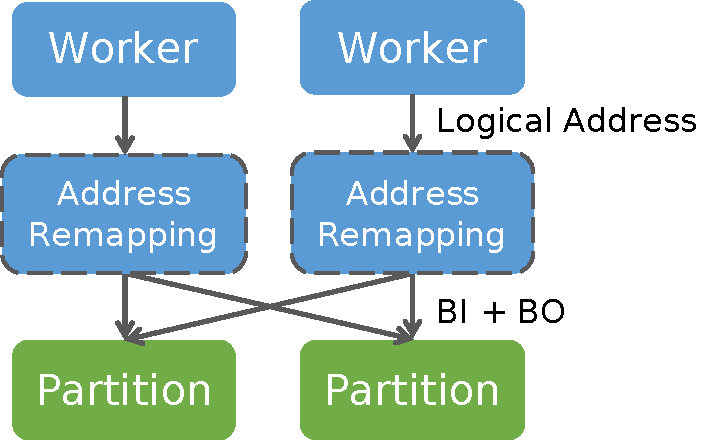
\includegraphics[width=1\columnwidth]{figs/spatialmemmodel.pdf}
  \caption{Reconfigurable Spatial Architecture}
  \end{subfigure}
  \caption[Memory model of different architectures]{Memory model of different architectures}
  \label{fig:memmodel}
\end{figure}
\begin{figure}
  \centering
  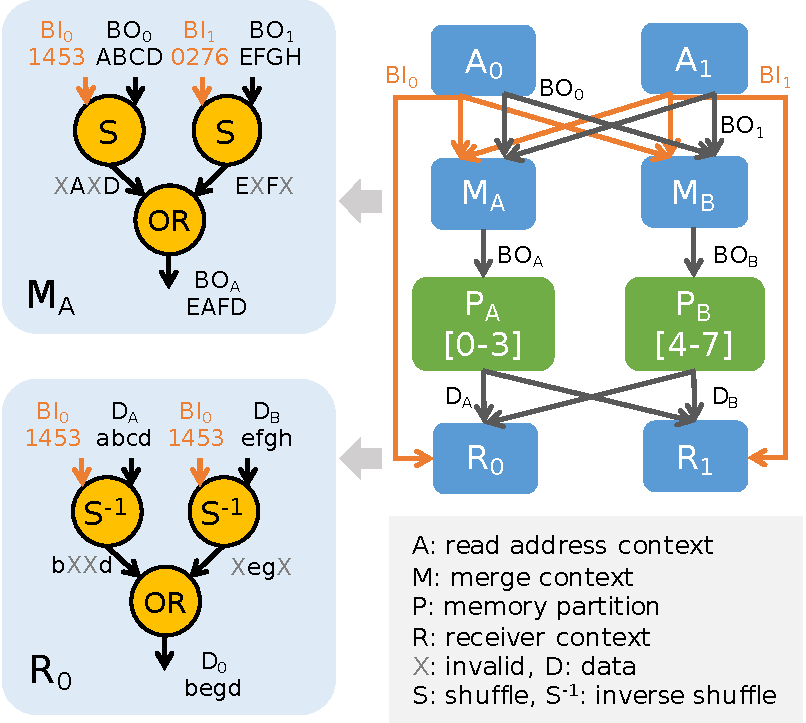
\includegraphics[width=0.6\columnwidth]{figs/memsplit2.pdf}
  \caption[Memory partitioning]{Example of memory partitioning across physical units. In this example, the program parallelizes the outer loop by two and vectorizes the inner loop by 4, which generates two vectorized access lanes. We need eight scratchpad banks to sustain the read bandwidth. 
  \name groups the 8 banks in two virtual memory partitions, $P_A$ (bank 0-3) and $P_B$ (bank 4-7). The address generation contexts $A_0$ and $A_1$ contains the computation for logical address and address remapping, which output $BA$s and $BO$s. \name allocates one merge context per memory partition
  ($M_A$ and $M_B$),
  merging requests from all access lanes. Inside the merge context, the shuffle operator converts the BO from access-aligned to bank-aligned. $A_0$, for example, requests offsets 
  A, B, C, and D ($BO_0$) from banks 1,4,5,and 3 ($BA_0$). The shuffle operator picks the requests belonging to partition A and outputs a BO aligned with bank 0-3. If the bank $i$ in the partition has no request, the $i$th element in the output is marked as invalid.
  The merge context contains one shuffle operator per request lane, and uses a tree of $OR$
  operators to combine all bank-aligned BOs into the final $BO_A$.
  On the receiver side, the memory broadcasts its response to all receiver lanes.
  The receiver context uses an inverse shuffle operator to convert the response from bank-aligned back to access-aligned, using the $BA$ forwarded from the address context. The response is then merged with another OR tree. 
  }
  \label{fig:memsplit}
\end{figure}

The coherence protocol is both expensive in hardware complexity and hard to scale in bandwidth for
streaming pipelined execution.
Instead of making redundant copies of the data, we can partition the data across different memory
partitions to get additional address port on a reconfigurable accelerator, as shown in
\Cref{fig:memmodel} (b).
Each parallel worker broadcasts the requests to all memory partitions.
If the data accessed by two parallel workers live in the same bank, the bandwidth will be halved.
To avoid bank conflicts, an important static analysis often used on reconfigurable accelerators is called static partitioning, or static banking~\cite{poly_cong}.
For most address patterns, the compiler can derive a partitioning scheme such that every partition is accessed by a
single worker at any time, which guarantees bandwidth at runtime.
The output of the analysis is an expression for bank address (BA) and bank offset (BO), both are
functions of the requested logical address.
BA determines which partition each request is going to, and BO is the offset within the
partition.

\Cref{fig:memsplit} shows how static banking is achieved on the Plasticine architecture.
Banking analysis from Spatial specifies the number of banks required to sustain bandwidth for the
current parallelization factors, and expressions for BAs and BOs. 
\name groups the banks into virtual memories, with group size limited by the number of banks in a PMU.
For each access lane, \name allocates a context to compute the logical and remapped address, which
outputs a vectorized BA and BO for each access lane. BAs and BOs are broadcasted to all memory partitions.
For each memory partition, \name allocates a merge context, merging BOs from all requesting lanes.
The merge context uses a shuffle operator to transform the vectorized BO from bank order specified by BA
(access-aligned) to bank order assigned to the current partition (bank-aligned).
Because the static banking analysis guarantees no bank conflicts for all banks,
\name can use a OR tree to merge the bank-aligned BOs into the final BO that gets send to
banks in the partition. On the receiver side, \name uses an inverse shuffle to convert responses from
partitions from bank-aligned back to access-aligned.
\name uses another OR tree to merge the access-aligned responses, which produces the final data
vector requested by the access lane.
With large parallelization, both the request OR tree and the respond OR tree can be
partitioned across VUs if running out of stages in a VU, scaling in the network bandwidth of the
crossbar connection by burning more VUs.

\Cref{sec:banking_arch} discusses the architectural changes to Plasticine to support this general
banking scheme.

\subsection{Register Allocation} \label{sec:regalloc}

After a VU is assigned to a PU, \name setups the configuration within a PU.
One of the configuration is assigning live variables in the dataflow graph to pipeline registers
across stages, shown in \Cref{fig:contexta}.

%\subsubsection{Blackbox IP Pruning} \label{sec:bbsplit}
%\yz{Cut this if out of the space}
%This step illustrates an example of integrating a customized partitioner for composable IP available on
%the architecture.
%The cost metrics and partition rule are specific to each IP.
%The example IP is a merge buffer, which can merge two sorted vector streams into a single stream with
%one vector per cycle throughput.
%The merge buffer pruner uses a tree of 2-way merge buffers across PUs to compose a multi-way merge buffer declared in the program.

\section{Optimizations}\label{sec:opt}
\name performs many of the standard compiler optimizations,
such as Dead Code Elimination and Constant Propagation.
Some of them, however, plays a much more important rule for reconfigurable accelerator because they
have direct impact on the resource usage.
Other optimizations can be counter-intuitive, as they introduce redundant computation that
reduces resource without necessarily impacting performance.
In this discussion, we focus our primary objective on performance.
Resource is an indirect objective as resource reduction enable larger parallelization factors,
, which in turn improves performance.

\subparagraph{Memory strength reduction (msr).} Like traditional strength reduction on arithmetics, \name{} replaces expensive on-chip memories with cheaper memories whenever possible.
%We map register accumulation in the program with single-cycle initiation interval to pipeline registers.
For example, \name{} replaces a scratchpad with constant address in all accesses to a un-indexable memory, such as a FIFO.
This commonly happens when producer and consumer loops of the memory are fully unrolled.

\subparagraph{Route-Through Elimination (rtelm).} For patterns where the content of a non-indexable memory  (M1) is read and written to another memory (M2), \name{} eliminates the intermediate access if the read of M1 and the write of M2 operates in lock-step.

\begin{figure*}
\centering
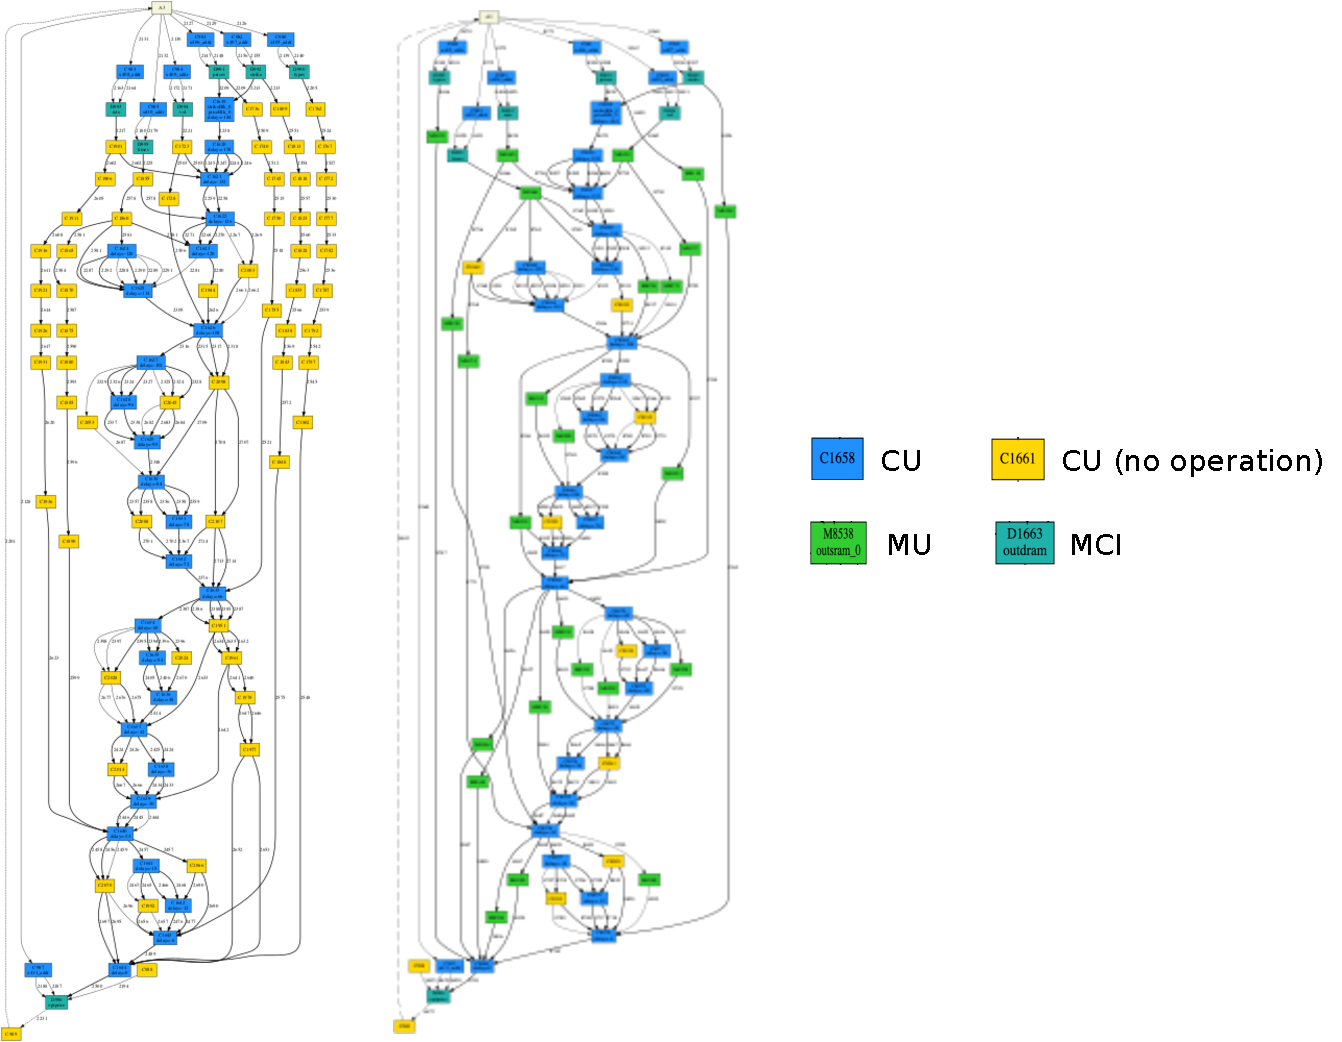
\includegraphics[width=0.7\textwidth]{figs/retiming.pdf}
\caption[Retiming]{
  Left: retiming with input buffer only. Right: retiming with either input buffer or scratchpad.
}
\label{fig:mlp}
\end{figure*}
\subparagraph{Retiming with scratchpad (retime-mem).} By default, \name{} uses PB input buffers for retiming purpose. 
This option enables \name{} to use scratchpad memory for retiming that requires large buffer depth.

\subparagraph{Crossbar datapath elimination (xbar-elm).}
Although, crossbars between accessors and memory partitions (\Cref{sec:memsplit}) are very expensive in the general case, the BI sometimes can be statically resolvable with certain combinations of parallelization on memory accesses. 
When BI is a constant, \name{} can use this information to intelligently assign virtual banks to partitions that reduce the crossbar data path to a partial or a point-to-point connection.

\subparagraph{Read request duplication (dupra).} During memory partitioning (\Cref{sec:memsplit}), instead of forwarding BI from the requester to receiver, \name{} can also duplicate the BI with local state on receiver side, which
eliminates the unbalanced data path at the cost of extra computation.

\begin{figure*}
\centering
\begin{subfigure}[b]{0.6\textwidth}
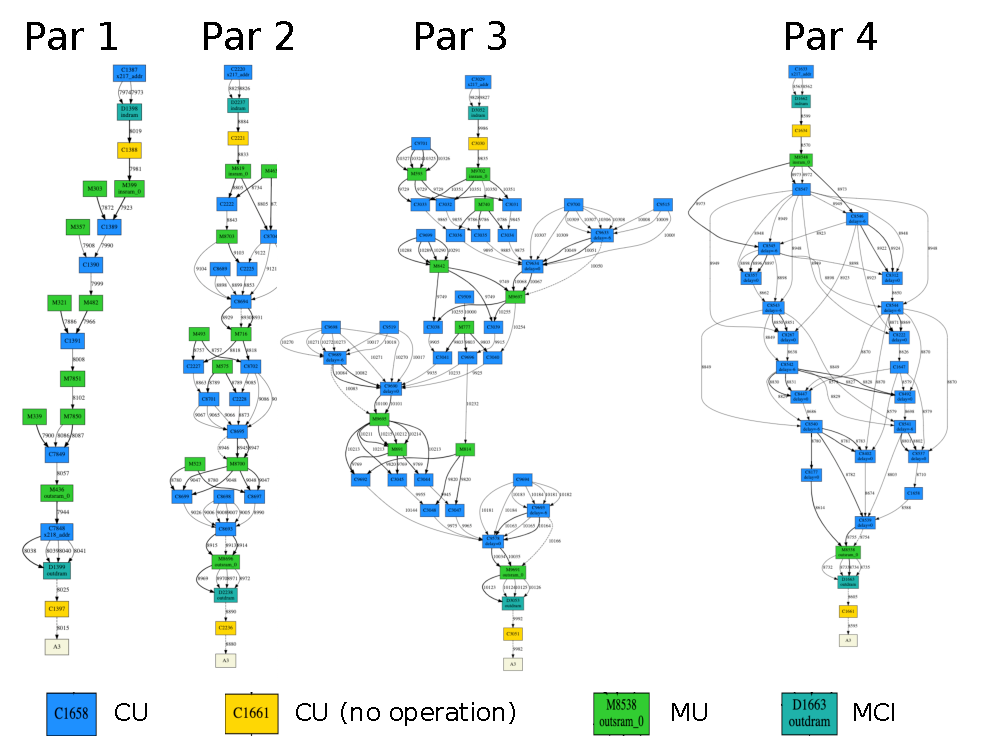
\includegraphics[width=1\textwidth]{figs/mlpunroll.pdf}
\caption{VUDFGs with different parallelization factors}
\end{subfigure}
\hfill
\begin{subfigure}[b]{0.39\textwidth}
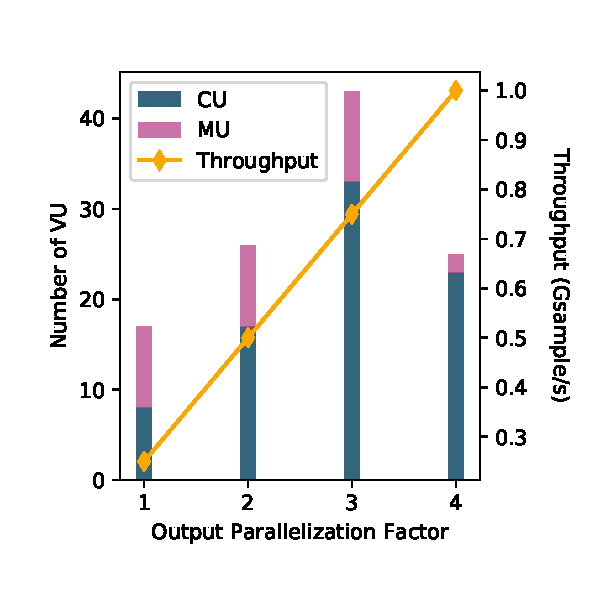
\includegraphics[width=1\textwidth]{figs/mlp.pdf}
\caption{Throughput and resource as a function of parallelization factor}
\end{subfigure}
\caption[MLP case study]{
  MLP case study
}
\label{fig:mlp}
\end{figure*}

\subparagraph{Global Merging (merge).}
After all VBs satisfy the hardware constraint, we perform a global optimization to compact small VBs into  larger VBs. 
Merging has very similar problem statement as compute partitioning (\Cref{sec:compsplit}) except with more constraints.
The traversal-based algorithm requires a reference cost for PB to check if the merged VB still satisfy the hardware constraint.
At each step of merging, we take the union of the domains of VBs within the current partition, and intersect with the domain of the merging VB.
The caveat is that even with a non-empty intersection, the bipartite graph might not have a possible assignment, as merged VB might fit in a larger PB with insufficient quantity.
Therefore, we perform a heuristic checking on feasibility of the bipartite assignment at each step of merging.
The solver-based solution combines partition assignment with PB type assignment as a joint problem. 
The output of merging gives both partition assignment as well as a PB type assignment, which eliminates the risk of un-mappable bipartite graph due to merging in the traversal-based solution.

\subparagraph{Memory Localization}
We perform another specialization on non-indexable memories (registers or FIFOs), whose all accesses have no explicit read enables.
Instead of treating them as shared memories, \name{} duplicates and maps them to local input buffers in all receivers, no longer requiring tokens.
The sender actor pushes to the network when the token is supposed to be sent, and the receiver dequeues one element from the input buffer when the token is supposed to be consumed.
This dramatically reduces the synchronization complexity of non-indexable memory in the common case.

\subparagraph{Reverse Loop Invariant Hoisting}
A common loop optimizations is to move loop invariant expressions outside of the loop body to reduce
computation. This optimizations, however, might introduce more basic blocks in the program.
For Plasticine, number of basic blocks have a strong correlation with number of contexts and
physical units. \Cref{fig:reversehoisting} shows an example where moving instructions into the loop
body reduces number compute units. Because instructions within basic blocks and basic blocks
themselves are pipelined, doing so does not have performance impact on the application.
Currently, we rely on the user to perform manually perform this optimization.

\begin{figure*}
\centering
\hfill
\begin{subfigure}[b]{0.4\textwidth}
\inputminted{python}{code/hoisting.py}
\caption{Input program}
\end{subfigure}
\hfill
\begin{subfigure}[b]{0.4\textwidth}
\inputminted{python}{code/reversehoisting.py}
\caption{Reverse Loop Invariant Hoisting}
\end{subfigure}
\hfill
\caption[Reverse Loop Invariant Hoisting]{
  The original program requires at least two contexts to execute Block 1 and Block 2.
  By moving the invariant instruction \texttt{c = a + b} into the loop body, (b) only needs a single
  context instead. Because instructions within \texttt{Block 2} are pipelined across loop
  iterations, adding instructions in the loop body introduce minimum performance impact.
  This transformation is beneficial until \texttt{Block 2} exceeds six operations, at which point
  both version consume the same amount of resources.
}
\label{fig:reversehoisting}
\end{figure*}

\begin{figure*}
\centering
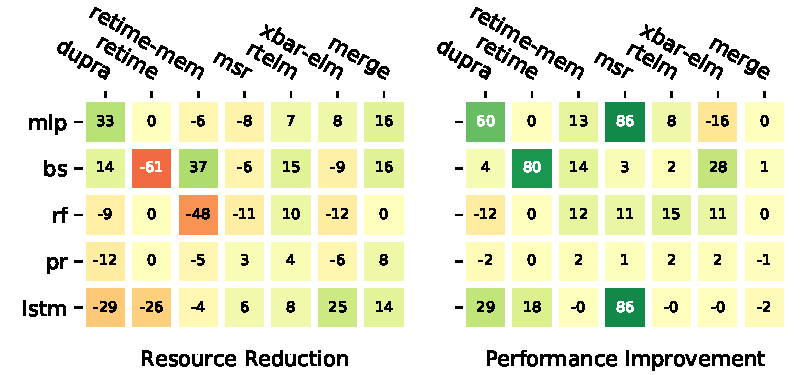
\includegraphics[width=0.7\textwidth]{figs/heat.pdf}
\caption[Optimization Effectiveness]{
  Optimization Effectiveness. Percentage resource reduction or performance improvement from each
  optimization. The heat map shows the maximum differences when turning on/off the optimization, 
  while keeping other optimizations the same.
  For a single application, the improvement is taking the geometric mean across different application parameters.
}
\label{fig:reversehoisting}
\end{figure*}

\begin{figure*}
\centering
\hfill
\begin{subfigure}[b]{0.35\textwidth}
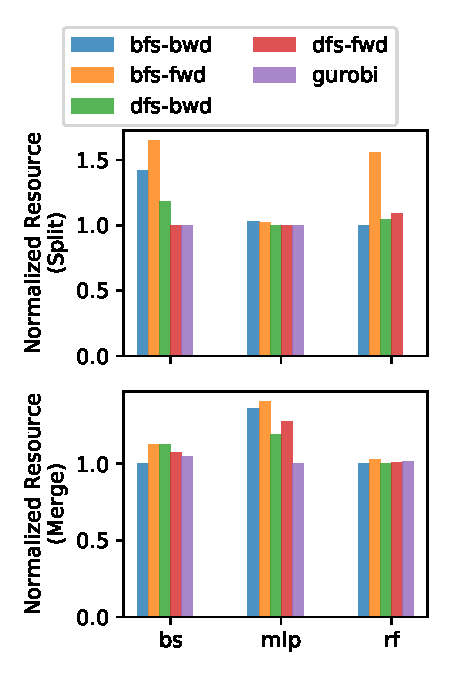
\includegraphics[width=1\textwidth]{figs/algo2.pdf}
\caption{Resource Comparison}
\end{subfigure}
\hfill
\begin{subfigure}[b]{0.64\textwidth}
\centering
\begin{tabular}{lccccc}
  \toprule
  Apps &bfs-bwd & bfs-fwd & dfs-bwd & dfs-fwd & gurobi \\ \midrule 
bs & 3s & 3s & 2s & 2s & 2h4m \\ 
mlp & <1s & <1s & <1s & <1s & 4s \\ 
rf & 1m37s & 1m7s & 29s & 27s & - \\ 

 \bottomrule
\end{tabular}
\caption{
  Compile time for spltting
}
\vspace{0.1cm}
\begin{tabular}{lccccc}
  \toprule
  Apps &bfs-bwd & bfs-fwd & dfs-bwd & dfs-fwd & gurobi \\ \midrule 
bs & 1s & 2s & 5s & 3s & 1m4s \\ 
mlp & 5s & 5s & 6s & 11s & 31m16s \\ 
rf & 11s & 10s & 2m7s & 1m0s & 14h27m \\ 

 \bottomrule
\end{tabular}
\caption{
  Compile time for merging
}
\vspace{0.65cm}
\end{subfigure}
\hfill
\caption[Partitioning and merging algorithm comparison]{
  Partitioning and merging algorithm comparison. (a) shows the normalized resource usage between
  different algorithms (the lower the better). (b) and (c) shows the compile time of each algorithm.
}
\label{fig:split}
\end{figure*}
%\subparagraph{Dead Code Elimination (DCE)} 
%We perform aggressive DCE on the VBDFG and only keeps computation that gets materialized to accelerator I/O and DRAM.
%\subparagraph{Constant Propagation}
%Aside from regular constant propagation on arithmetics, we also eliminates crossbar datapath when bank ID 
%can be statically resolved described later in \Cref{sec:memsplit}.
%During loop unrolling, address of indexable memory sometimes can be resolved to static constant.
%For a read-only RAM with constant address, we lookup their content at compile time and embed its content into registers.
%For \emph{route-through} pattern, where content of a non-indexable memory M1 is read and written to another memory M2,
%we can eliminate the intermediate write and forward the data directly to the final memory if the compiler
%can prove the read M1 and write of M2 operates in lock-step.
%We also perform constant propagation on control signals with loop-range analysis. 
%Eliminates the control signals can expose more lock-step accesses and \emph{route-through} opportunities.
%\subparagraph{Strength Reduction}
%In addition to traditional strength reduction on arithmetics, we also replace expensive memories
%with cheaper memory whenever possible.
%We map register accumulation in the program with single-cycle initiation interval to pipeline registers.
%Banked-SRAM with constant bank IDs and offsets in all accessors can also be replaced with FIFOs,
%which is happens when producer and consumer loops are fully unrolled.

%Accesses statically banked in the input graph can operates concurrently 
%without bank conflicts, as explained in \Cref{sec:background}.
%These accesses are usually from a unrolled loops. For banked accesses from the same pre-unrolled access, 
%\name first merge all requests before sending to the memory (details in \Cref{sec:memsplit}). 
%Because these accesses are from loop unrolling, they have the same program order and same dependency with other accesses.
%So the synchronization can be performed on the merged access, which prevents the amount of synchronization
%to increase with parallelism on a banked memory, as shown in \Cref{fig:mergetoken}

%\subsubsection{Blackbox IP Pruning} \label{sec:bbsplit}
%\yz{Cut this if out of the space}
%This step illustrates an example of integrating a customized partitioner for composable IP available on
%the architecture.
%The cost metrics and partition rule is specific to each IP.
%The example IP is a merge buffer, which can merge two sorted vector streams into a single stream with
%one vector per cycle throughput.
%The merge buffer pruner uses a tree of 2-way merge buffers across PBs to compose a multi-way merge buffer declared in the program.



\section{Placement and Routing} \label{sec:par}
The input to the \emph{placement and routing (PaR)} phase is a VUDFG, with each VU tagged to a PU
type.
Before PaR, \name also performs a runtime analysis of the program, annotating each edge in the VUDFG
with a link priority. The link priority is used to determine the routing order during PaR.
PaR then iteratively places VUs and route edges in VUDFG onto the global network.

In addition to the original static network in Plasticine, we introduce a dynamic network in
parallel to the static network, forming a dynamic-static hybrid network.
Both purely static and purely dynamic networks are instances of the parameterized hybrid network.
\Cref{sec:network} will discuss the details about the hybrid network.
The PaR algorithm needs to handle both network types and multiple network granularity (vector,
scalar, control) at the same time.

The major difference between the static and the dynamic network is that each physical link in the static network is dedicated to a logical edge in the VUDFG for the entire duration of the execution
(circuit-switching\footnote{Technically, our static network is more restrictive than
circuit-switching because circuit-switching allows deallocation after the connection is terminated.
Our static network, on the other hand, cannot be reconfigured until the application terminates.}), whereas 
the physical link in the dynamic network can be time-shared by multiple logical edges
(packet-switching).
Both static and dynamic networks are statically routed by the PaR algorithm. 
For a dynamic network, PaR also needs to assign virtual channels (VCs) to prevent network deadlock.
The PaR algorithm configures the lookup table in each router that maps the packet header to the
destination port and VC.

In the rest of this section, \Cref{sec:place} and \Cref{sec:route} discusses the placement 
and the routing algorithm. 
\Cref{sec:vc} explains the need for VC allocation. 
Lastly, \Cref{sec:heuristic} describes how \name generates link priority.

\subsection{Iterative Placement} \label{sec:place}

At high-level, the PaR algorithm works very similarly to the FPGA PaR using
simulated annealing~\cite{simanneal}. 
For the initial placement, the algorithm places VUs in VUDFG in topological order.
Each VU is placed to the next available PU with minimum Manhattan distance to the placed
neighbors of that VU.
Next, the algorithm routes all edges in the VUDFG, starting from edges with the highest link
priority. If no routes are available on the static network, the route will be moved onto the dynamic
network. For purely static networks, there is an ``imaginary'' dynamic network for this step.
If there are still routes on the fake dynamic network at the end of the PaR, PaR is considered
failed for the purely static network.
After all routes are routed, either on the static or dynamic network, the PaR evaluates the
congestion cost of the current placement.
Then, a genetic algorithm shuffles the VUs whose edges contribute most to congestion, 
and keeps the new position if it improves the route assignment.
By iteratively re-placing and re-routing, the mapping process eventually converges to a good placement.

The PaR uses a heuristic cost model to rapidly evaluate placements: a 
penalty score is assigned as a linear function of several subscores.
These include projected congestion on dynamic links, projected congestion at network injection and ejection ports, the average route length, and the length of the longest route.
\name provides a static estimate of the number of packets sent on each logical link.
The PaR algorithm estimates congestion by normalizing the number of packets on each link to the program link with the highest total packet count.
The most active program link sets a lower bound on the program runtime (the highest bandwidth physical link can still only send one packet per cycle), which translates to an upper bound on congestion for other links.

%The {\sc Unplace} function randomly decides between unplacing a random node, and unplacing one or several nodes based on heuristics.
%For the heuristic-based unplacement, a node's contribution to global route congestion is calculated by adding an estimate of all connected routes' contributions to the global penalty score; the node(s) with the highest scores are unplaced.
%Similarly, {\sc Place} also can either randomly place an unplaced node, or place it to minimize the Manhattan distance to its logical neighbors. {\sc Score} calculates the heuristics for each node, and {\sc Filter} duplicates the best candidate placements to fill the pool. Because the unplacement and replacement steps can make a placement worse, the best performing placements are frozen in each iteration to ensure that no good placements are thrown away.

\subsection{Congestion-Aware Routing} \label{sec:route}
%\info{Somewhere we should mention that placement and routing running interchangeably}
To achieve optimal performance, we use a routing algorithm that projects congestion and routes around it. 
Routing starts with the highest-priority routes, as determined by fanout of the broadcast edge and
estimated packet count; broadcast edge with higher fanout is harder to route and hence are routed
first.
Using the packet count as a priority makes sure that the static network is used most efficiently.
Our scheme searches a large space of routes for each link, using Dijkstra's algorithm \cite{dijkstra} and a hop weighting function.
To ensure maximum link reuse in broadcast edges, we can augment the hop weight in Dijkstra's
algorithm by a multiplication factor between zero and one. 
When finding the shortest path between each source-destination pair, the weight of the hop is
multiplied by the factor each time the hop is reused for the same broadcast edge.
In other words, the reused path has a lower hop cost compared to other paths.
This trick provides a balance between the shortest path and link reuse: a smaller factor encourages link
reuse, even though individual source-destination pairs are not the shortest path; a factor equals to 1 ensure all source-destination pairs are routed with the shortest path.
The second objective for routing broadcast links is balancing the hop counts between all
destinations. This is because the shorter path will back pressure the sender before packets reaching to the longer path, causing pipeline stalls.
To achieve this, we start with the source-destination pair with the longest Manhattan distance, ensuring
the most far apart source-destination pair is routed on the shortest path.
The consecutive source-destination pairs will try sharing the link on this path and slightly detour from
their shortest path, which balances the hop count.
%Routes are not analyzed on the basis of a single source-destination pair, which would be inadequate for broadcasts: instead, a directed graph is built from the source and all destinations in the route, with edge weights corresponding to the minimal route between each pair of VUs in the broadcast.
%For example, if the broadcast is from VU-1 to VU-2 and VU-3, four total potential routes are analyzed for congestion: VU-1 to VU-2, VU-1 to VU-3, VU-2 to VU-3, and VU-3 to VU-2.
%The routes are weighted so that routes mapped on the static network are preferable to those mapped to the dynamic network; within these categories, routes are weighted based on length. 

%\info{does the nodes refer to only source and destinations or including all nodes on the path between source and destination. How does the weights represent the minimum routes? Is it capturing the cost of the minimum route?}
%Then, a search algorithm based on Prim's algorithm for minimum spanning trees \cite{prim1957shortest} is run to build a tree for the broadcast, starting with only the source being reached.
%At every step, the most-preferable route (from the graph built using Dijkstra's algorithm) that adds a new destination VU to the reached set is chosen and added to the broadcast, until all destination VUs are reached. 
%This route can start from either the source of the broadcast tree or any destination currently in the reached set.
%The algorithm will find a fully static broadcast tree, if one exists, and will only add a non-static route to the broadcast (moving the entire broadcast to the dynamic network) when there are VUs in the tree that cannot be reached from the source VU by \emph{any} static route.
%\info{does the algorithm routes links from high priority to low from all nodes or it does one node at a time?}

\subsection{VC Allocation for Deadlock Avoidance} \label{sec:vc}
Deadlock is a system pathology in dynamic routing where multiple flits form a cyclic holds on/waits for dependency on each others' buffers and prevent forward progress.
Most dataflow accelerators use a streaming model, where outputs of a producer are sent over the network to one or more consumers
without an explicit request; the producer is backpressure when there is insufficient buffer space. 
While this paradigm improves accelerator throughout by avoiding the round-trip delay of a request-response protocol, it introduces an additional source of deadlock \cite{hansson2007avoiding}. 

\Cref{fig:deadlock}(a) shows a sample VUDFG graph, which is statically placed and routed on a $2\times3$ network in (b). 
Logical edges B and C share a physical link in the network. If C fills the buffer shared with B, VU-3 will never receive any packets from B and will not make forward progress.
%For y-z dimension-order routing, the only valid routes from VU-1 to VU-3 is through $\[0,1\], \[0,0\], \[1,0\], \[2,0\]$. 
%Dimension-order routing prevents deadlock by eliminating cycles in network routes.
%On traditional NoCs, deadlock can be solved with dimension-order routing, which routes all traffic on one dimension before another.
%\yaqi{
  With streaming computation, the program graph must be considered as part of the network dependency graph, which must be cycle-free to guarantee deadlock freedom. However, this is infeasible because cycles can exist in a valid VU dataflow graph when the original program has a loop-carried dependency. Therefore, deadlock avoidance using cycle-free routing, such as dimension-order routing, does not work in our scenario. 
Allocating VCs to prevent multiple logical links from sharing the same physical buffer is consequently the most practical option for deadlock avoidance on streaming accelerators.
%Because the entire program is connected through these streaming dependencies, any two links can conflict and result in a deadlock.
%\yaqi{However, cycles are permitted in the programming paradigms since loop-carried dependencies can be mapped across the network.
%Therefore, we perform VC allocation at each router to prevent multiple logical links from sharing the same physical buffer.
\if 0
Virtual channel (VC) allocation is another common approach to avoid deadlock. We can statically assign conflicting streams B and C with different
virtual channels at router $[2,0]$, which prevents them to share physical buffers. 
Notice indirect inputs of a VU, such as A and D with eventual consumer VU-3,
also need distinct VCs to ensure deadlock-free. To minimize the number of VCs required, we perform per-hop VC allocation--statically
assign conflicting links at each input of each router with distinct VCs. The VCs can be looked up at runtime based on link ID.
Distinct links from the same source VU, such as A and C, can share the same VC because VU-1 ensures the number of flits sent over A and C remains
to a ratio that the receiver expects, which permits data to drain in the network.
\fi

\begin{figure}
\centering
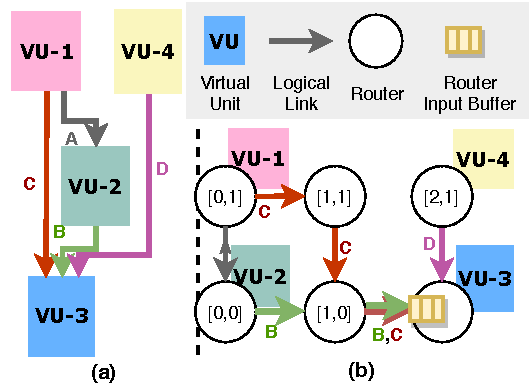
\includegraphics[width=0.4\columnwidth]{figs/deadlock.pdf}
  \caption[Network deadlock in streaming accelerators]{An example of deadlock in a streaming accelerator, showing the (a) VU data-flow graph and (b) physical placement and routes on a $2\times3$ network. There are input buffers at all router inputs, but only the buffer of interest is shown.}\small\textsuperscript{}\label{fig:deadlock}
\end{figure}

\subsection{Runtime Analysis for Heuristic Generation} \label{sec:heuristic}

In Spatial, users can annotate the value of runtime variables to assist compiler analysis.  
We use these programmer annotations to compute the expected number of iterations each basic block
will execute. 
The execution count on the basic block can further be used to derive the packet counts produced
by these basic blocks.
For a loop with data-dependent bounds, the user can annotate an estimate of the bound value.
For a branch statement, the user can annotate a percentage distribute between the if and else clauses.
The runtime of a streaming program is a function of the number of packets received on the incoming
stream. 
Static runtime analysis can identify potential application-level deadlock due to stream mismatching, as shown
in \Cref{fig:runtime}.

The derived packet counts based on these annotations can help the placer to evenly spread out the traffic.
The placer prioritizes highly used links on the static network and leaves infrequently used links on the dynamic network. 
However, we do not require exact annotations for efficient placement---rough estimates of these runtime values are sufficient to determine the relative importance of links.
When no annotation is provided, the compiler estimates
loop iteration counts based on the nesting depth: packets generated by the innermost loops are 
the more likely to be frequent.
This heuristic provides a reasonable estimate of links' priorities for routing purposes.

\begin{figure*}
\centering
\begin{subfigure}[b]{0.8\textwidth}
\inputminted{python}{code/runtime.py}
\caption{Example program}
\end{subfigure}
\caption[Runtime analysis]{
  Example of a streaming program whose runtime depends on the number of packets received on
  \texttt{stream}. We use a \texttt{queue} to model a stream receiving the packets from the
  network.
  Loop \emph{A} is a forever loop whose runtime is determined by its child controllers.
  With user annotation on number of packets from \texttt{stream}, 
  we know the runtime of loop \emph{B} is $T(B) = N$.
  As a result, we can derive the runtime of loop \emph{B}'s and parent \emph{A}, 
  i.e. $T(A) = \lceil\frac{N}{B}\rceil$. 
  With runtime for $A$, the runtime for $C$,$D$,and $E$ can be computed as
  $T(C) = \lceil\frac{N}{B}\rceil\cdot C$,
  $T(D) = \lceil\frac{N}{B}\rceil\cdot C \cdot R$, 
  and $T(E) = \lceil\frac{N}{B}\rceil\cdot C \cdot R \cdot E$.
  The runtime for \emph{E} also depends on \texttt{q}, which gives $T(E) = T(B) = N$. 
  If $\lceil\frac{N}{B}\rceil\cdot C \cdot R \cdot E \neq N$, \name gives an warnning for the
  inconsistency that potentially triggers an undesired deadlock.
}
\label{fig:runtime}
\end{figure*}

%\section{Debugging and Instrumentation Support (WIP)}
%\subsubsection{Deadlock in Streaming Reconfigurable Architecture}

%\subsubsection{Debugging Support and Performance Instrumentation}

\section{Evaluation (WIP)} \label{sec:eval}

\begin{figure*}
\centering
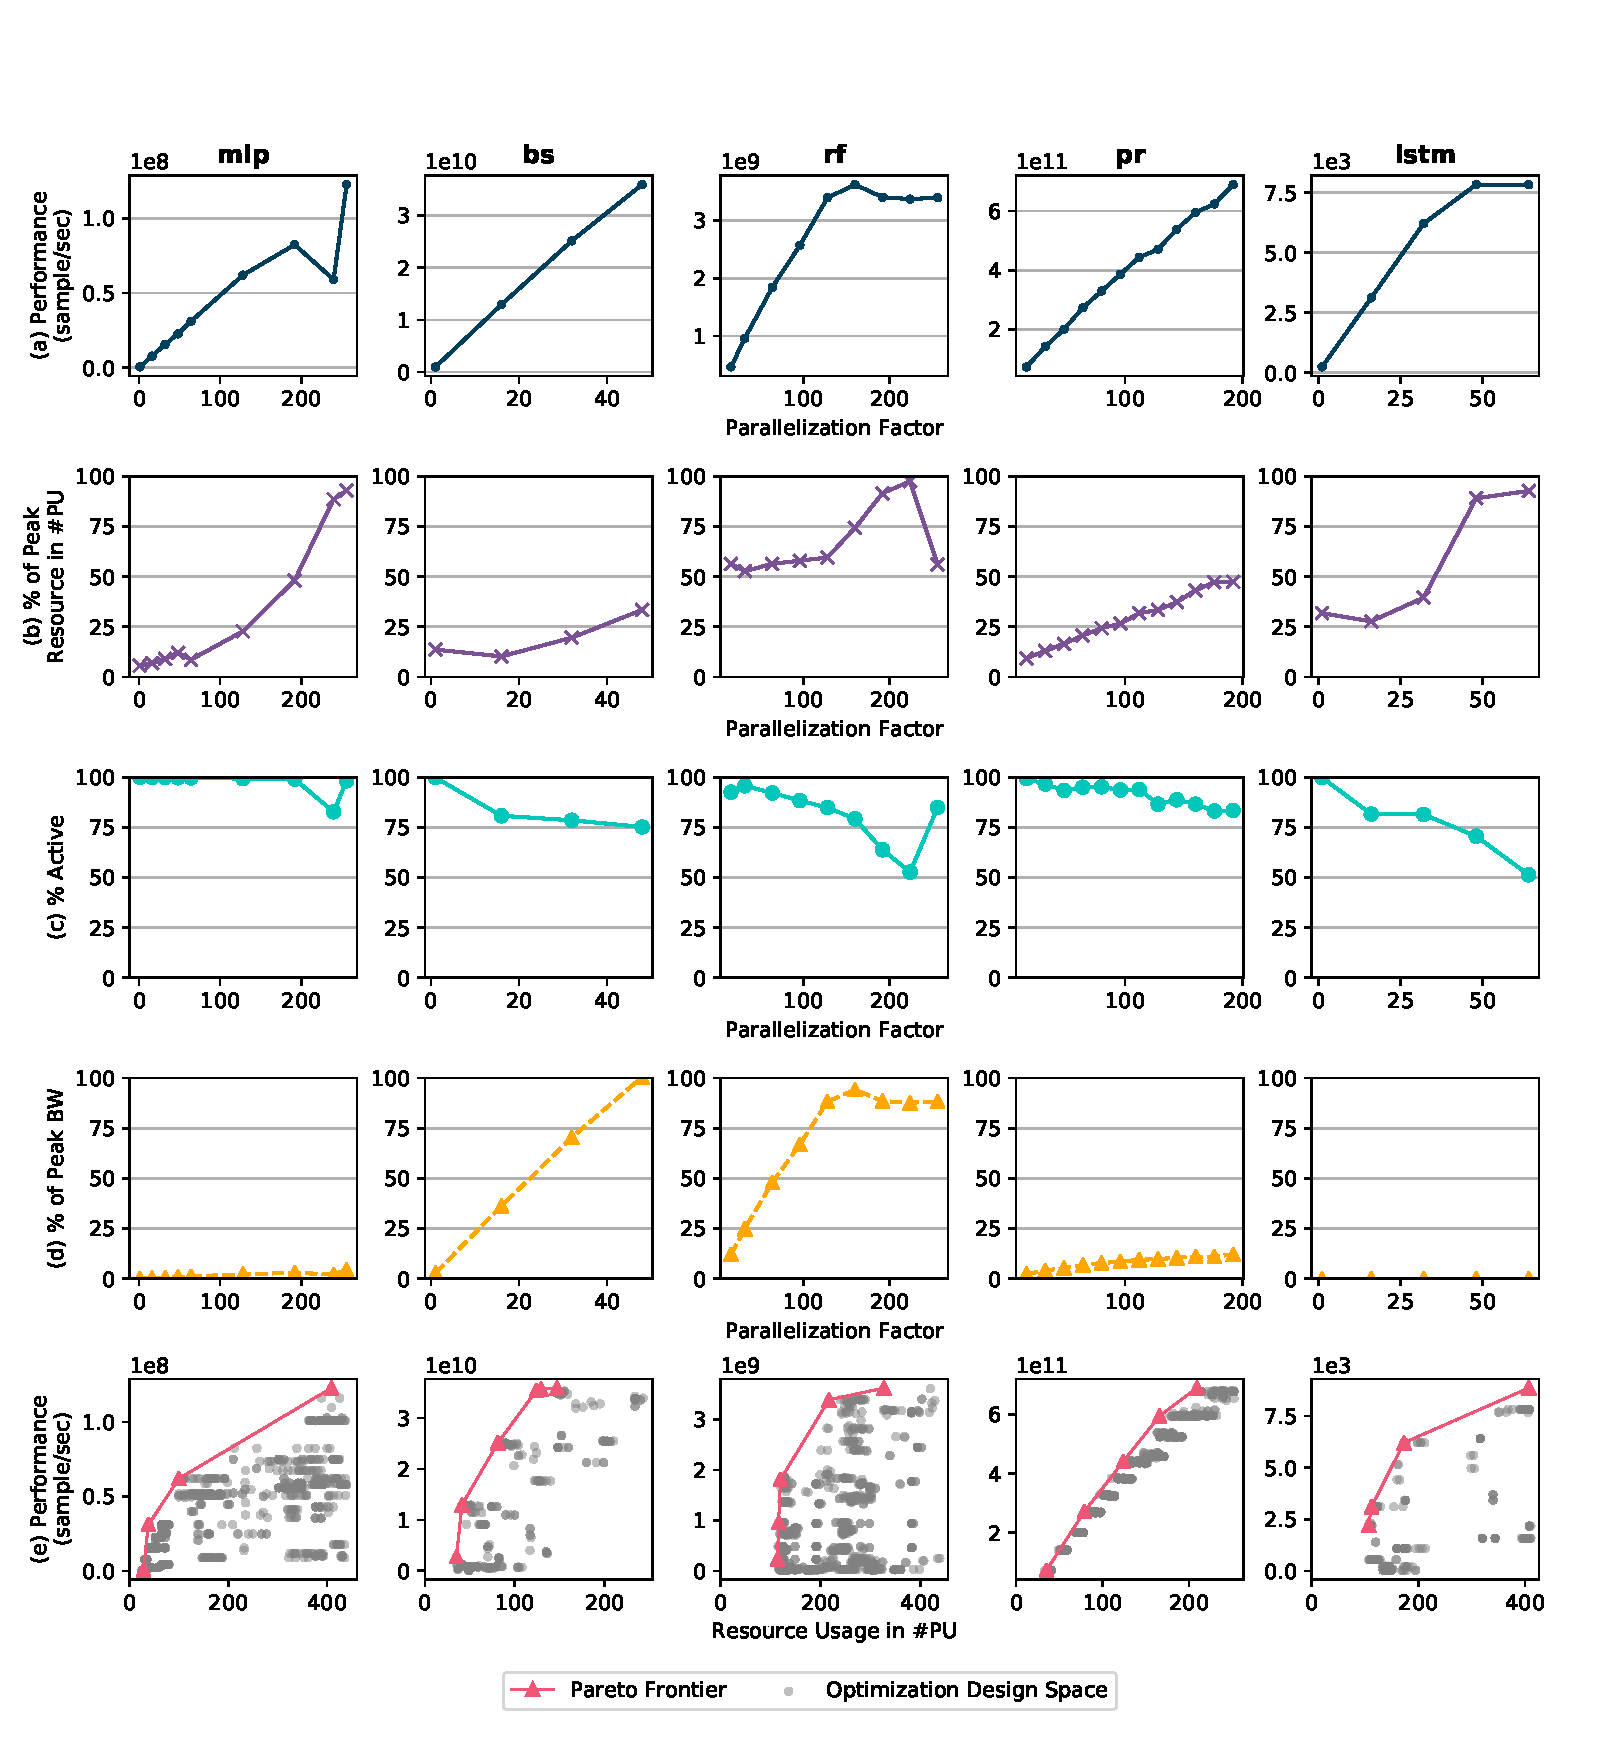
\includegraphics[width=1\textwidth]{/Users/yaqiz/pldi20/paper/figures/par_thesis.pdf}
\caption[Scalability Evaluation]{
  Scalability Evaluation. 
  The first four charts show the scaling of
  (a) throughput, 
  (b) resource usage, 
  (c) runtime activation rate of PUs on the critical path of the compute pipeline, 
  and (d) achieved HBM bandwidth, as the program gets parallelized.
  (e) shows the combined design space of compiler optimizations and parallelization factors on a
  throughput-resource curve. 
  The pareto frontier presents the throughput shown in (a) as a function of resource increase in
  (b).
}
\label{fig:par}
\end{figure*}

%\begin{figure*}
%\centering
%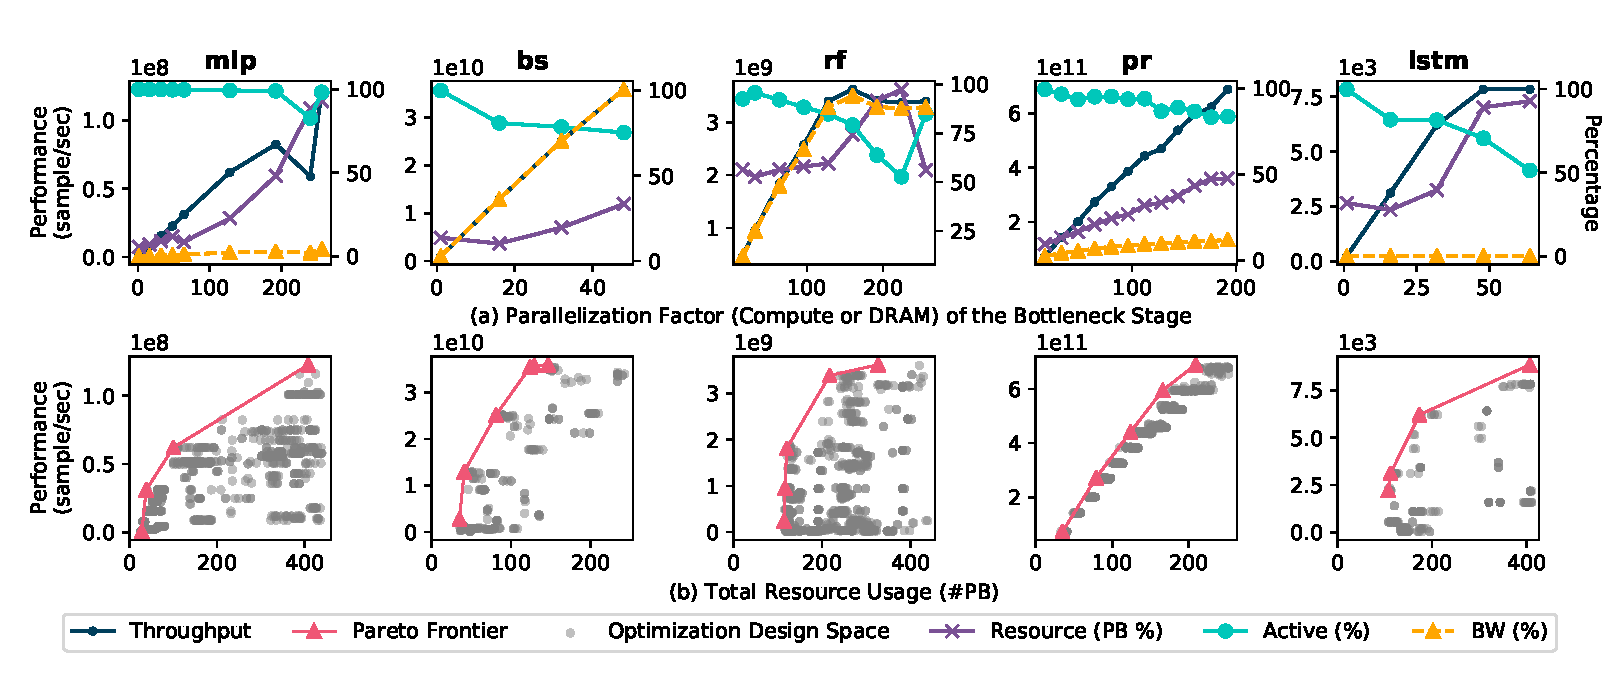
\includegraphics[width=1\textwidth]{/Users/yaqiz/pldi20/paper/figures/par.pdf}
%\caption[Performance comparison with V100 GPU]{
%}
%\label{fig:par}
%\end{figure*}

\begin{table}[t]
  \centering
    \footnotesize
    \begin{tabular}{lcccccc}
    \toprule
      \multirow{2}{*}{\textbf{Benchmark}} &
      \multirow{2}{*}{\makecell[c]{\bf Throughout\\\bf Unit}} &
      \multirow{2}{*}{\makecell[c]{\bf GPU\\\bf Compiler}} & \multicolumn{2}{c}{\textbf{Latency} (ms)} &
      \multicolumn{2}{c}{\textbf{Throughput} (Unit/s)} \\
                                & & & \name & GPU & \name & GPU     \\
      \midrule
        SqueezeNet (batch-1) & {\em kFrames}   & TF+cuDNN & 49.13  & 70.10  & 0.12 (1.1) & 0.4   \\ \addlinespace
        LSTM (batch-32)      & {\em kSamples}  & TF+cuDNN & 3.61   & 6.81   & 8.8 (79.2) & 4.7   \\ \addlinespace
        PageRank             & {\em MEdges}    & GunRock & 128.27 & 829.39 & 49         & 7.5   \\ \addlinespace
        BlackScholes         & {\em GOptions}  & CUDA & 0.09   & 0.10   & 88.88      & 80.02 \\ \addlinespace
        Random Forest        & {\em MSamples}  & CUDA & 0.10   & 0.32   & 1.04       & 0.32  \\ \addlinespace
        Merge Sort           & {\em GElements} & CUDA & 0.63   & 2.14   & 6.65       & 1.96  \\
      \bottomrule
    \end{tabular}
  \caption{Performance comparison of Plasticine with Tesla's V100 GPU (Normalized throughput to transistor count in parentheses).}
  \label{tab:gpu-comparison}
\end{table}
\begin{figure*}
\centering
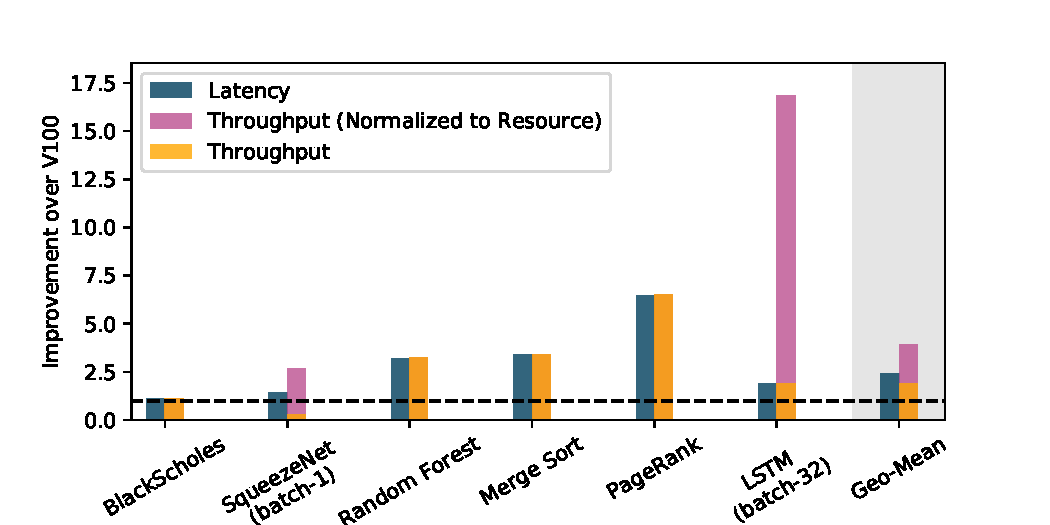
\includegraphics[width=1\textwidth]{figs/slide_gpu.pdf}
\caption[Performance comparison with V100 GPU]{
  Plasticine's latency and throughout improvement over V100 GPU.
  The evaluated Plasticine architecture has area footprint of 352$mm^2$ at 28nm.
  V100 GPU has area footprint of 815$mm^2$ at 12nm.
  Both platforms have the same off-chip bandwidth at 1TB/s with HBM technology.
  Yellow and blue bars show the raw measured speedup in throughput and latency, respectively.
  To account for the resource discrepancy, the pink bar shows the normalized throughput
  for compute-bound application--SqueezeNet and LSTM, which scales performance with additionally
  on-chip resources.
}
\label{fig:peakutil}
\end{figure*}

